\documentclass[10pt, t, xcolor={usenames,dvipsnames,svgnames}, compress]{beamer}

\usepackage{hyperref}
\usepackage{booktabs}
\usepackage{dcolumn}
\usepackage{colortbl}
\usepackage{ifxetex}
\usepackage{amsmath}
\usepackage{mathtools}
\usepackage[backend=bibtex,style=authoryear-icomp, maxcitenames=2,hyperref=true]{biblatex}

\definecolor{untractable_red}{RGB}{209, 25, 25}
\definecolor{tractable_green}{RGB}{0, 153, 51}

\usetheme{enziteto}


\setbeamertemplate{headline}{}

\definecolor{lacamdarklilac5} {RGB} {51, 10, 102}
\definecolor{lacamgold5} {RGB} {255, 87, 0}
\definecolor{violet} {RGB} {119, 111, 178}
\definecolor{petroil2} {RGB} {36, 165, 175}
\definecolor{petroil4} {RGB} {30, 132, 149}
\definecolor{petroil6} {RGB} {23, 101, 115}
\definecolor{gold2} {RGB} {255, 130, 0}
\definecolor{gold4} {RGB} {250, 100, 0}
\definecolor{gold6} {RGB} {245, 90, 0}

\AtEveryCite{\color{violet}\bf}

\newcommand{\argmax}{\operatornamewithlimits{argmax}}
\newcommand{\highlight}[2][yellow]{\mathchoice%
  {\colorbox{#1}{\textcolor{white}{$\displaystyle#2$}}}%
  {\colorbox{#1}{\textcolor{white}{$\textstyle#2$}}}%
  {\colorbox{#1}{\textcolor{white}{$\scriptstyle#2$}}}%
  {\colorbox{#1}{\textcolor{white}{$\scriptscriptstyle#2$}}}}%

\addbibresource{../referomnia/referomnia.bib}


\title{Learning Sum-Product Networks}
\author{\small Nicola Di Mauro \and Antonio Vergari}
\date{\scriptsize International Conference on Probabilistic Graphical Models\\
 Lugano, Switzerland, 6-9 September 2016}
\institute{\scriptsize Università degli Studi di Bari}
\department{Dipartimento di Informatica}
\laboratory{\scriptsize LACAM}
\group{Machine Learning}
\institutelogo{
\includegraphics[width=25pt]{figures/unibaba}}
\lablogo{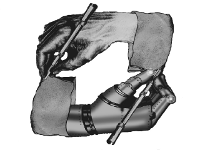
\includegraphics[width=35pt]{figures/lacam}}

%\footnotesize \let\small\footnotesize

\renewcommand*{\thefootnote}{[\arabic{footnote}]}

\setbeamerfont{footnote}{size=\scriptsize}
%\addtobeamertemplate{footnote}{}{\vspace{16pt}}
\newcommand{\customcite}[1]{\footnote{\scriptsize \citeauthor{#1}, \citetitle{#1}, \citeyear{#1}}}
\newcommand{\customcitenomark}[1]{\footnotenomarkleft{\scriptsize \citeauthor{#1}, \citetitle{#1}, \citeyear{#1}}}

\begin{document}

\begin{frame}[c]
  \setbeamertemplate{headline}{}
  \setbeamertemplate{footline}{}
  \titlepage
\end{frame}

\begin{frame}
\frametitle{The need for Tractable Inference}

Probabilistic modeling of data aims at
\begin{itemize}
  \item representing probability distributions \emph{compactly}
  \item computing their marginals and modes \emph{efficiently} (inference)
  \item learning them \emph{accurately}
\end{itemize}
A solution is to use Probabilistic Graphical Models (PGMs)
%$P(X) = \frac{1}{Z}\prod_k \phi_k(x_{\{k\}})$
%with $Z = \sum_x \prod_k \phi_k(x_{\{k\}})$.

However, PGMs are limited in
\begin{itemize}
\item representing compact distributions
\item having intractable (exponential in their treewidth) exact inference in the worst case 
  \begin{itemize}
  \item falling back on approximate inference
  \end{itemize}
\item requiring and exponential sample size (wrt the number of variables)
\item learning the structure since it requires inference
\end{itemize}
Exact inference in a tractable model may be better than performing approximate
inference in an intractable model
\end{frame}

\begin{frame}
  \frametitle{The need for SPN }
  \framesubtitle{Why should you work on SPNs?}

Sum-Product Networks (SPNs) are a type of probabilistic model\customcite{Poon2011}
\begin{itemize}
\item a class of deep probabilistic  models  that  consist  of  many  layers  of
  hidden variables and can have unbounded treewidth\\ 
  \hfill {\color{violet} \textbf{$\rightarrow$ probabilistic semantics and NN interpretation}}
\item inference in SPNs is guaranteed to be tractable
\begin{itemize}
\item structure and parameters can be effectively and accurately learned
\end{itemize}
\end{itemize}
SPNs represent probability distributions and a corresponding exact inference
machine for the represented distribution at the same time 
\end{frame}


\section{Representation}
{\setbeamertemplate{headline}{}
  \begin{frame}[c]
    \sectionpage
  \end{frame}
}

\begin{frame}
  \frametitle{Density estimation}

Given a set of i.i.d. samples $\{\mathbf x_i\}_{i=1}^N$ over RVs $\mathbf{X}$, the aim is to
learn an estimator for the joint probability distribution  $p_{\mathbf{X}}$
% representation of a distribution as normalized product of factors
% $$P(\mathbf X = \mathbf x) = \frac{1}{Z}\prod_k \phi_k(\mathbf x_{\{k\}})$$
% with $Z = \sum_x\prod_k \phi_k(\mathbf x_{\{k\}})$ the partition function
\bigskip
%\vskip 0.5cm

{\color{lacamdarklilac5} \textbf{Unsupervised learning density estimators}}
\begin{itemize}
  \item Bayesian Networks
  \item Markov Networks
  \item Kernel Density Estimators
  \item \ldots
\end{itemize}\bigskip

SPNs have been introduced as a general architecture efficiently encoding an
unnormalized probability distribution $p_{\mathbf X}$ over a set of random 
variables


\end{frame}

\begin{frame}
  \frametitle{(Different kinds of) Inference}
  Different types of models make different operations tractable

\vskip 10pt

Operations that may be required to be efficient are
  \begin{itemize}
  \item $p(\mathbf{X} = \mathbf{x})$ (evidence)\\
    \hfill {\color{violet} $\rightarrow$ tractable for SPNs, BNs}
  \item $p(\mathbf{E}), \mathbf{E}\subset\mathbf{X}$ (marginals)\\
    \hfill {\color{violet} $\rightarrow$ tractable for SPNs, hard in
      BNs (even approximate)}
  \item $p(\mathbf{Q}|\mathbf{E}), \mathbf{Q},
    \mathbf{E}\subset\mathbf{X}, \mathbf{Q}\cap \mathbf{E}=\emptyset$
    (conditionals)\\
    \hfill \hfill {\color{violet} $\rightarrow$ tractable for SPNs,
      hard in BNs (even approximate)}
  \item
    $\arg\max_{\mathbf{q}\sim\mathbf{Q}}p(\mathbf{q}|\mathbf{E})$
    (MPE assignment)\\
    \hfill {\color{violet} $\rightarrow$ hard for both SPNs and BNs}
  \item $Z =\sum_{\mathbf{x}\sim \mathbf{X}}\phi(\mathbf{x})$
    (partition function)\\
    \hfill {\color{violet} $\rightarrow$ tractable for SPNs, hard
    for MNs}
    \item sampling: generate independent samples from the posterior distribution
  \end{itemize}
\end{frame}

\begin{frame}
  \frametitle{Tractable Probabilistic Models}
Due to the importance of efficient inference a lot of work has been devoted to
learning probabilistic models for which inference is guaranteed to be tractable 
\begin{itemize}
\item Graphical models
  \begin{itemize}
  \item  graphical models with low treewidth and their mixtures
  \item thin junction trees
  \end{itemize}
\item Computational graphs from Knowledge Compilation
\begin{itemize}
\item Arithmetic Circuits
\item Sentential Decision Diagrams\customcite{Darwiche2009}
\end{itemize}
\item Neural Networks
\begin{itemize}
\item Restricted Boltzmann Forest 
\item Neural Autoregressive Distribution Estimator (NADE)\customcite{Larochelle2011}
\item Masked Autoencoder Distribution Estimator (MADE)\customcite{Germain2015}
\end{itemize}
\end{itemize}
\end{frame}

\begin{frame}
  \frametitle{Sum-Product Networks}
  A \emph{Sum-Product Network} $S$ over RVs $\mathbf X$ is a
  rooted weighted DAG consisting of
  distribution \emph{\color{violet}\textbf{leaves}} (network inputs),  \emph{\color{violet}\textbf{sum}} and \emph{\color{violet}\textbf{product}}
  nodes (inner nodes).

\vspace{0.5 cm}
\begin{minipage}{0.65\textwidth}
\begin{itemize}
\item  A leaf $n$ defines a tractable, possibly unnormalized, distribution
  $\phi_{n}$ over some RVs in $\mathbf X$.
\item  A nonnegative weight $w_{nc}$ is associated to each edge linking a sum node
  $n$ to $c\in\mathsf{ch}(n)$
\begin{itemize}
\item $\mathsf{ch}(n)$:  child (input) nodes of   a node $n$ 
\item $\mathsf{pa}(n)$:  parent (output) nodes of a node $n$
\item $S_{n}$: sub-network rooted at node $n$ 
\end{itemize}
\end{itemize}
\end{minipage}
\begin{minipage}{0.3\textwidth}
\centering
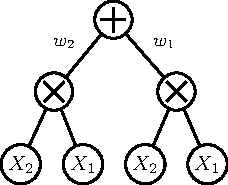
\includegraphics[width=0.9\columnwidth]{figures/spn-mixture.pdf}
\end{minipage}
\end{frame}

\begin{frame}
  \frametitle{Scopes}
\begin{minipage}{0.55\textwidth}
  The \emph{\color{violet}\textbf{scope}} of a node $n$ in $S$ is denoted as
  $\mathsf{sc}(n)\subseteq\mathbf{X}$
\begin{itemize}
\item   the scope of a leaf node $n$ is defined as the set of RVs over which
  $\phi_{n}$ is defined
\item the scope of an inner node $n$ is defined as
  $\mathsf{sc}(n)=\bigcup_{c\in\mathsf{ch}(n)}\mathsf{sc}(c)$
\item the scope of $S$ is the scope of its root, i.e. $\mathbf{X}$
\end{itemize}
\end{minipage}
\begin{minipage}{0.44\textwidth}
\begin{center}
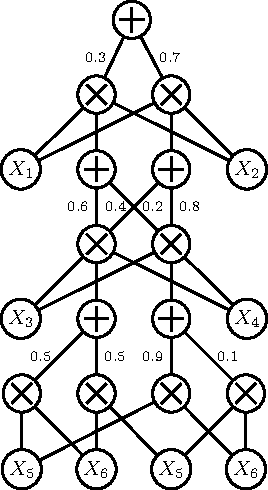
\includegraphics[width=0.7\columnwidth]{figures/spn-eval.pdf}
\end{center}
\end{minipage}
\end{frame}


\begin{frame}
  \frametitle{Structural Properties}
  Let $S$ be an SPN and let $\mathbf S_{\oplus}$ (resp. $\mathbf S_{\otimes}$) be the set of all sum
  (resp. product) nodes in $S$
\begin{enumerate}  
\item    $S$ is \emph{\color{violet}\textbf{complete}} iff $\forall n\in
  \mathbf S_{\oplus},\forall c_{1}, c_{2}\in \mathsf{ch}(n):
  \mathsf{sc}(c_{1})=\mathsf{sc}(c_{2})$
\item    $S$ is \emph{\color{violet}\textbf{decomposable}} iff $\forall n\in
  \mathbf S_{\otimes},\forall c_{1}, c_{2}\in \mathsf{ch}(n), c_{1}\neq c_{2}:
  \mathsf{sc}(c_{1})\cap\mathsf{sc}(c_{2})=\emptyset$
\item    If $S$ is complete and decomposable, then it is \emph{\color{violet}\textbf{valid}} \customcite{Darwiche2009}\customcite{Poon2011}
\end{enumerate}  

Evaluating a valid network corresponds to
evaluate a joint unnormalized probability distribution
$p_{\mathbf{X}}$: $\forall\mathbf{x},S(\mathbf{x})/Z=p(\mathbf{X = x})$
\begin{itemize}
\item $Z$ being the normalizing \emph{partition} function 
$Z=\sum_{\mathbf{x}\sim \mathbf{X}}S(\mathbf{x})$
\end{itemize}\bigskip

Valid SPN correctly compiles the
\emph{extended network polynomial} encoding
the distribution $p_{\mathbf{X}}$~\customcite{Peharz2015a}.

\end{frame}


\section{Inference}
{\setbeamertemplate{headline}{}
  \begin{frame}[c]
    \sectionpage
  \end{frame}
}




\begin{frame}
\frametitle{Complete evidence inference}

\begin{minipage}{0.4\linewidth}
  \vspace{10pt}
  \begin{center}
    \only<1>{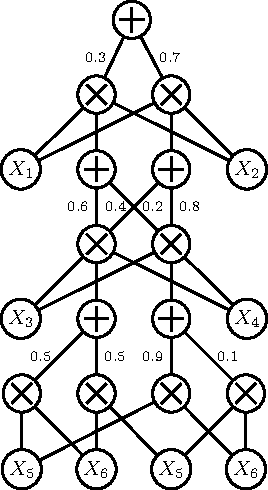
\includegraphics[width=0.75\columnwidth]{figures/spn-eval.pdf}}
    \only<2>{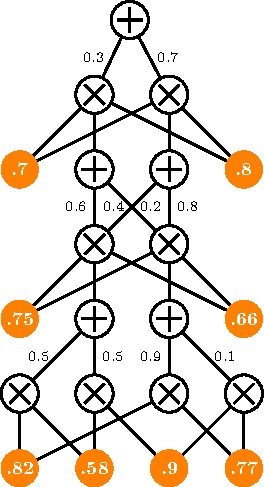
\includegraphics[width=0.75\columnwidth]{figures/spn-eval-ev-1}}
    \only<3>{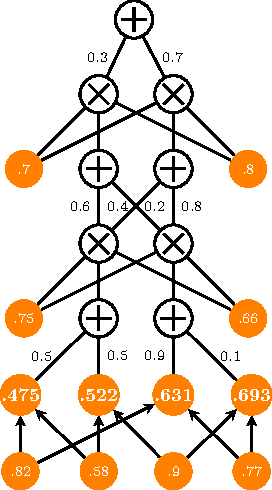
\includegraphics[width=0.75\columnwidth]{figures/spn-eval-ev-2}}
    \only<4>{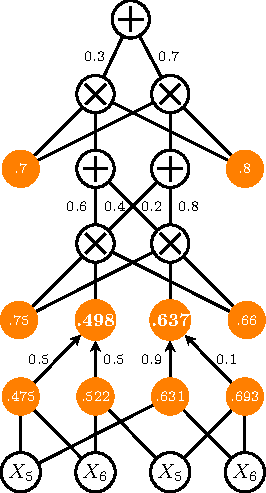
\includegraphics[width=0.75\columnwidth]{figures/spn-eval-ev-3-s}}
    \only<5>{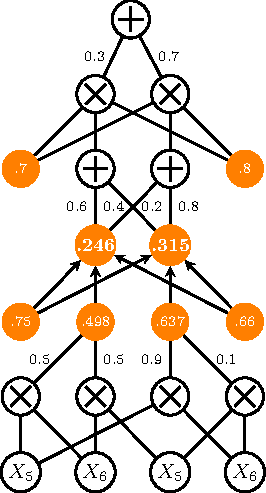
\includegraphics[width=0.75\columnwidth]{figures/spn-eval-ev-4-s}}
    \only<6>{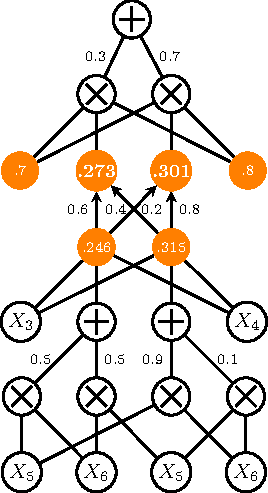
\includegraphics[width=0.75\columnwidth]{figures/spn-eval-ev-5-s}}
    \only<7>{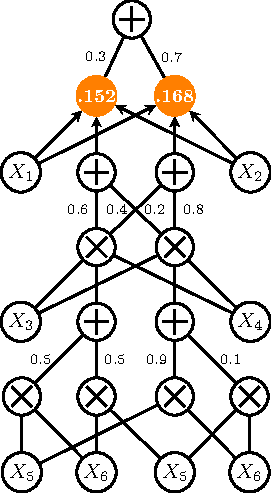
\includegraphics[width=0.75\columnwidth]{figures/spn-eval-ev-6-s}}
    \only<8>{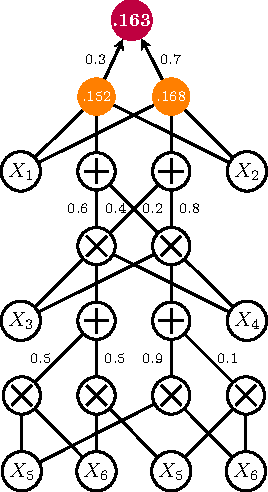
\includegraphics[width=0.75\columnwidth]{figures/spn-eval-ev-7-alt-s}}
  \end{center}
\end{minipage}\hfill\begin{minipage}[t]{0.58\linewidth}
  \vspace{-80pt}
  To compute $p(\mathbf{X}=\mathbf{x})$, evaluate nodes in a bottom-up (feedforward)
  fashion.\par\bigskip
  Each node $n$, compute $S_{n}(\mathbf{x}_{|\mathsf{sc}(n)})=S_{n}(\mathbf{x})$:
  \begin{itemize}
  \item<2-8> $S_{n}(\mathbf{x}) = \phi_{n}( \mathsf{sc}(n)
    =\mathbf{x}_{|\mathsf{sc}(n)})$\par if $n$ is a leaf node
  \item<3-8> $S_{n}(\mathbf{x}) =\prod_{c\in
      \mathsf{ch}(n)}S_{c}(\mathbf{x})$\par if $n$ is a
    product node
  \item<4-8> $S_{n}(\mathbf{x}) =\sum_{c\in
      \mathsf{ch}(n)}w_{nc}S_{c}(\mathbf{x})$\par
    if $n$ is a sum node
  \end{itemize}
  % \only<5-8>{iteratively traversing children before parents}
  % \only<6-8>{\dots}\only<7-8>{\dots}\only<8>{ up to the root
  %   output is
  %   \colorbox{purple}{\textcolor{white}{$S(\textbf{x})=p(\mathbf{X}=\mathbf{x})$}}}
  \only<8>{ the root output is \colorbox{purple}{\footnotesize\textcolor{white}{$S(\textbf{x})=p(\mathbf{X}=\mathbf{x})$}}}
\end{minipage}
\end{frame}



\begin{frame}
  \frametitle{Marginal inference}

Exact marginal inference can be computed with the same time complexity if the
validity property holds\customcite{Poon2011}

To compute a marginal query like $p(\mathbf{Q=q}),
\mathbf{Q}\subset\mathbf{X}$, one has to evaluate each leaf $n$ as:
\begin{equation}
  \label{eq:marg}
  S_{n}(\mathbf{q}) = \begin{cases}
    p(\mathsf{sc}(n) =\mathbf{q}_{|\mathsf{sc}(n)}) & \text{if $\mathsf{sc}(n)\subseteq\mathbf{Q}$} \\
    1 & \text{otherwise}
  \end{cases}
\end{equation}
and then propagate the outputs as before

\begin{itemize}
\item each sub-network shall output 1 as the probability of marginalizing
over all the RVs out of its scope
\end{itemize}

Even conditional probability queries are also computable
in tractable time
$$p(\mathbf{Q}|\mathbf{E}) = p(\mathbf{Q}, \mathbf{E})/p(\mathbf{E})$$

\end{frame}

\begin{frame}
\frametitle{Marginal Inference}
\framesubtitle{Example}
\begin{minipage}{0.49\textwidth}
\onslide<1-3>{
    \only<1-3>{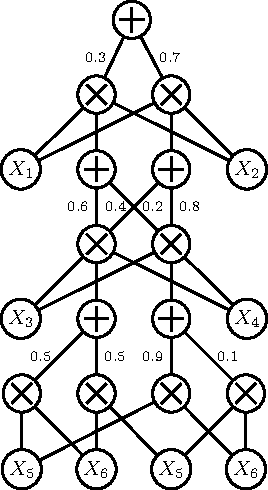
\includegraphics[width=0.6\columnwidth]{figures/spn-eval.pdf}}
}
\end{minipage}
\begin{minipage}{0.49\textwidth}
    \only<2>{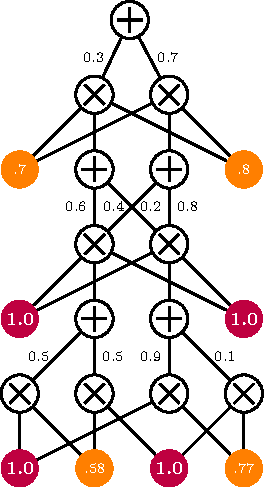
\includegraphics[width=0.6\columnwidth]{figures/spn-eval-marg-1-alt.pdf}}
    \only<3>{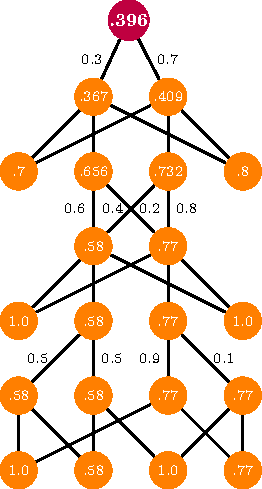
\includegraphics[width=0.6\columnwidth]{figures/spn-eval-marg-2-alt.pdf}}
\end{minipage}
\end{frame}



\begin{frame}
  \frametitle{MPE inference}
An approximation of MPE inference can be answered in linear time as
well\customcite{Peharz2015b}\customcite{Peharz2016}

\begin{equation}
\mathbf{q}^{*}=\argmax_{\mathbf{q}\sim \mathbf{Q}}p(\mathbf{E},
\mathbf{q})
\label{eq:mpe-ass}
\end{equation}
for some RVs $\mathbf{E}, \mathbf{Q} \subset\mathbf{X},
\mathbf{E}\cap\mathbf{Q}=\emptyset, \mathbf{E}\cup \mathbf{Q}=\mathbf{X}$

\begin{itemize}
\item a Max-Product Network $M$ is built by substituting each $n\in \mathbf S_{\oplus}$ for a max node computing
$\max_{c\in\mathsf{ch}(n)}w_{nc}M_{n}$
\item $M$ is evaluated bottom-up after setting all leaves $n$, $\mathsf{sc}(n)\subseteq
\mathbf{Q}$, to output 1
\item a top-down traversal traces back the MPE
assignment for each RV in $\mathbf{Q}$
\item starting from the root and following only the max output
child branch of a max node and all the child branches
of a product node\customcite{Poon2011a}, each instance determines a
\emph{tree} path whose leaves MPE assignments union forms the
query answer\customcite{Darwiche2009}
\end{itemize}
\end{frame}

\begin{frame}
\frametitle{MPE Inference}
\framesubtitle{Example}
\begin{center}
\onslide<1-5>{
    \only<1>{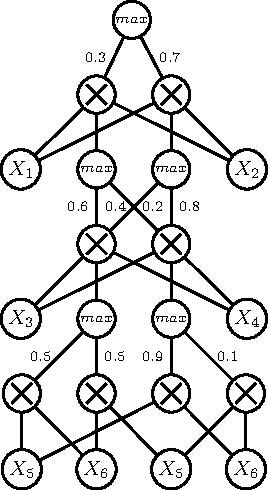
\includegraphics[width=0.33\columnwidth]{figures/spn-eval-mpe-1.pdf}}
    \only<2>{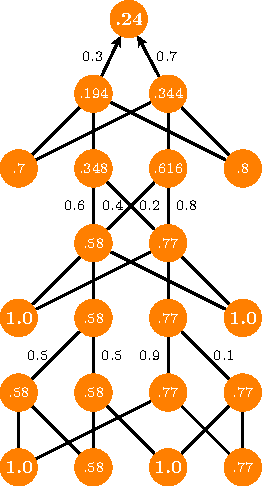
\includegraphics[width=0.33\columnwidth]{figures/spn-eval-mpe-2.pdf}}
    \only<3>{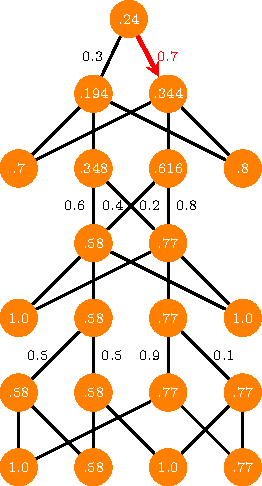
\includegraphics[width=0.33\columnwidth]{figures/spn-eval-mpe-3.pdf}}
    \only<4>{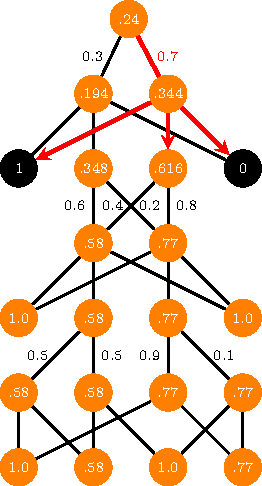
\includegraphics[width=0.33\columnwidth]{figures/spn-eval-mpe-4-alt.pdf}}
    \only<5>{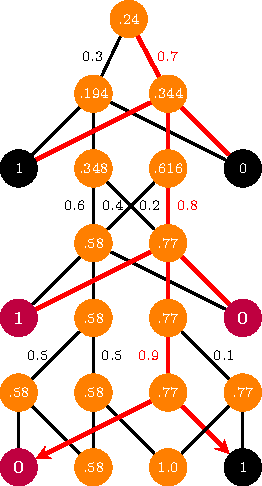
\includegraphics[width=0.33\columnwidth]{figures/spn-eval-mpe-5-alt.pdf}}
}
\end{center}
\end{frame}

\begin{frame}
\frametitle{Partition function}
\framesubtitle{Example}
As for ACs, setting all leaf outputs to 1 equals to compute the \emph{partition function} 

\begin{center}
\onslide<1-2>{
    \only<1>{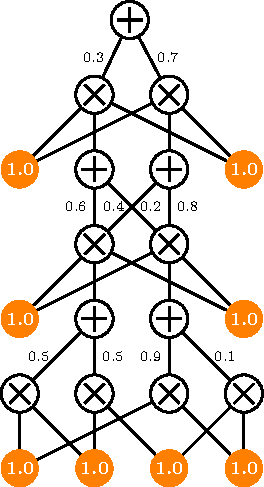
\includegraphics[width=0.33\columnwidth]{figures/spn-eval-part-1.pdf}}
    \only<2>{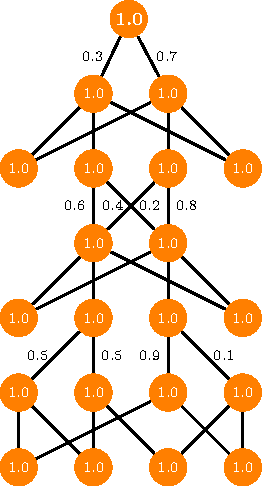
\includegraphics[width=0.33\columnwidth]{figures/spn-eval-part-2.pdf}}
}
\end{center}
\end{frame}


\section{Interpretation}
{\setbeamertemplate{headline}{}
  \begin{frame}[c]
    \sectionpage
  \end{frame}
}

\begin{frame}
\frametitle{SPN interpretations}
{\color{lacamdarklilac5}\textbf{Probabilistic model}}
\begin{itemize}
\item sum nodes in a valid network are probabilistic mixtures over their
  children distributions whose coefficients are the children weights 
\begin{itemize}
\item a categorical latent RV $H_n$ can be associated to each sum node $n$,
  having values in $\{1,\ldots, |\mathsf{ch}(n)|\}$
\item the weights of a sum node $n$ can also be interpreted as the probabilities
  of choosing the corresponding child branch from node $n$, having already taken
  the path from the root up to $n$
\end{itemize}
\item since product nodes are evaluated as product of probability
values, they identify factorizations over independent distributions  
\end{itemize}
{\color{lacamdarklilac5}\textbf{Deep feedforward neural network}}
\begin{itemize}
\item SPNs  can  also  be  interpreted  as  a  particular  kind  of  feedforward  deep  Neural
Networks  (NNs)  with  nonnegative  parameters,  where  the  leaf  distributions
are input neurons whereas sum and product nodes are the hidden neurons
\end{itemize}
\end{frame}

\begin{frame}
  \frametitle{SPNs and other models}
  \begin{itemize}
  \item SPNs are more general than both hierarchical mixture models and thin
    junction trees
    \begin{itemize}
    \item SPNs can be exponentially more compact (distribution over states of variables
      with an even number of 1’s, for instance)
    \end{itemize}
  % \item SPNs can be viewed as probabilistic, general-purpose convolutional
  %   networks, with average-pooling corresponding to marginal inference and
  %   max-pooling corresponding to MPE inference 
  % \item Like  deep  belief  networks,  SPNs  can  be used for nonlinear
  %   dimensionality reduction,  and allow objects to be reconstructed from the
  %   reduced representation
  \item SPNs are not classical PGMs
  \item SPNs are not ``probabilistic, general-purpose convolutional
    networks, with average-pooling corresponding to marginal inference and
    max-pooling corresponding to MPE inference''
  \end{itemize}
\end{frame}


\begin{frame}
\frametitle{Network Polynomials}

Let $\Phi(x) \geq 0$ an unnormalized probability distribution on Boolean
variables.

$x$ (resp. $\bar{x}$) denotes the indicator function $[x]$ (resp. $[\bar{x}]$) for
the variable $X$.

The network polinomial\customcite{Darwiche2003} of $\Phi(x)$ is $\sum_x \Phi(x) \Pi(x)$
\begin{itemize}
\item $\Pi(x)$ is the product of the indicators that have value 1 in state $x$
\end{itemize}
\begin{example}[Bernoulli distribution over $X$ with parameter $p$]
$$px + (1-p)\bar{x}$$
\end{example}
\begin{example}[Bayes Network $X_1 \rightarrow X_2$]
$$\theta_{x_1}\theta_{x_2|x_1}x_1x_2 +
\theta_{x_1}\theta_{\bar{x}_2|x_1}x_1\bar{x}_2 + 
\theta_{\bar{x}_1}\theta_{x_2|\bar{x}_1}\bar{x}_1x_2 +
\theta_{\bar{x}_1}\theta_{\bar{x}_2|\bar{x}_1}\bar{x}_1\bar{x}_2$$
with $\theta_{\cdot}=P(\cdot)$ 
\end{example}
\end{frame}

\begin{frame}
\frametitle{Network Polynomials (II)}
\begin{itemize}
\item The  network  polynomial  is  a  multilinear  function  of  the indicator
variables
\item The  unnormalized  probability  of  evidence $e$  (partial  instantiation  of $X$) 
is  the  value  of  the network  polynomial  when  all  indicators  compatible  with
$e$ are set to 1 and the remainder are set to 0

\begin{example}
$\Phi(X_1 = 1, X_3= 0)$ is the value of the network polynomial
when $\bar{x}_1$ and $x_3$ are set to 0 and the remaining indicators
are set to 1 throughout.
\end{example}

\item The partition function is the value of the network polynomial when all
indicators are set to 1

\item For any evidence $e$, the cost of computing $P(e) = \Phi(e)/Z$
is linear in the size of the network polynomial

\item The network polynomial has size exponential in the number
of variables

\item {\color{red}it is possible to represent and evaluate it
in polynomial space and time using an AC or an SPN}
\end{itemize}
\end{frame}

\begin{frame}
  \frametitle{Arithmetic Circuits}
Arithmetic Circuits (ACs)\customcite{Darwiche2003}: inference representation closely related to SPNs
\begin{itemize} 
\item a rooted DAG with sums and products as interior nodes
\item indicator nodes and parameters as leaves
\end{itemize}
Properties
\begin{itemize}
\item \emph{\color{violet}\textbf{decomposable}}: children of a product node have disjoint scopes
\item \emph{\color{violet}\textbf{smooth}}: children of a sum node have identical scopes
\item \emph{\color{violet}\textbf{deterministic}}: children  of  a  sum  node  are  mutually  exclusive
\begin{itemize}
\item at most one is non-zero for any complete configuration
\end{itemize}
\end{itemize}

An  AC  represents  a  valid  probability  distribution  if  it  is decomposable
and smooth

ACs generated by compiling graphical models are typically deterministic as well
\begin{itemize}
\item while for SPNs  sum nodes represent mixtures of distributions and are not
deterministic in general
\end{itemize}

\end{frame}


\begin{frame}
  \frametitle{Arithmetic Circuits (II)}

ACs and SPNs representations are equivalent for discrete
domains\customcite{Rooshenas2014}
\begin{itemize}
\item every decomposable and smooth AC can be represented as an equivalent SPN
with fewer or equal nodes and edges
\item every  SPN  can  be represented as an AC with at most a linear increase in
  the number of edges
\end{itemize}
Learning ACs has been made by
\begin{itemize}
\item a standard BN structure learner with the complexity of the
  resulting circuit as the regularizer\customcite{Lowd2012}
\item learning MNs representable by ACs, but does not
  reusing sub-ACs\customcite{Lowd2013}
\end{itemize}

SPN learning algorithms emphasize mixtures
\begin{itemize}
\item results in models that use implicit latent variables to
capture all of the interactions among the observable variables
\end{itemize}
%\item AC learning methods are based on learning  algorithms PGM  without  hidden
%  variables 
%\begin{itemize}
%\item no searching within the sum-product network structure
%\end{itemize}

\end{frame}

\begin{frame}
  \frametitle{Arithmetic Circuits (II)}
  \framesubtitle{Differences with SPNs}

{\color{lacamdarklilac5}\textbf{probabilistic semantics of SPNs}}
  \begin{itemize}
  \item allows for direct structure learning schemes where the compilation
    process is implicit
  \item allows sampling from their encoded distribution (generative model)
  \end{itemize}
  {\color{lacamdarklilac5}\textbf{no shared weights}}
\begin{itemize}
\item differently from ACs, it is not possible to have the same tied parameter
  for many nodes in SPNs
\end{itemize}
{\color{lacamdarklilac5}\textbf{generalized SPNs}}
\begin{itemize}
\item instead of using IVs to represent the states of discrete RVs, SPNs have been
  generalized to continuous RVs and discrete RVs with infinitely many states\customcite{Peharz2015a}
\begin{itemize}
% \item IVs can be interpreted as discrete distribution assigning all probability
%   mass to a single state
\item IVs $\lambda_{X=x}$ are replaced by distributions
\end{itemize}
\end{itemize}
\end{frame}

\begin{frame}[t]
  \frametitle{SPNs as NNs (I)}
  SPNs are a particular kind of \emph{\textbf{labelled}
    \textbf{constrained} and \textbf{fully probabilistic}}
  neural networks.\par\bigskip
  
  \textbf{Labelled}: each neuron is associated a \emph{scope}\par
  \textbf{Constrained}: completeness and decomposability determine
  network topology.\par
  \textbf{Fully probabilistic:} each valid sub-SPN is still a
  valid-SPN.\customcitenomark{Vergari2016a}\par\bigskip
  
  SPNs provide a direct encoding of the input space into a deep
  architecture $\rightarrow$ \emph{\textbf{visualizing representations}} (back) into the \emph{\textbf{input space}}.
\end{frame}

\begin{frame}
  \frametitle{SPNs as NNs (II)}
  \small
  A classic MLP hidden layer computes the function:
  $$h(\mathbf{x}) =\sigma(\mathbf{W}\mathbf{x}+ \mathbf{b})$$

  SPNs can be reframed as \textit{DAGs} of MLPs, each sum layer
  computing:
  $$\mathbf{S}(\mathbf{x}) =
  \log(\mathbf{W}\mathbf{x})$$
  and product layers computing:
  $$\mathbf{S}(\mathbf{x}) = \exp(\mathbf{P}\mathbf{x})$$
  where
  $\mathbf{W}\in\mathbb{R}_{+}^{s\times r}$ and $\mathbf{P}\in\{0,
  1\}^{s\times r}$ are the weight matrices:
  \begin{equation*}
    \mathbf{W}_{(ij)}= \begin{cases}
      w_{ij} &\text{if $i\rightarrow j$}\\
      0& \text{otherwise}
    \end{cases}\quad\quad\mathbf{P}_{(ij)}=
    \begin{cases}
      1 &\text{if $i\rightarrow j$}\\
      0& \text{otherwise}
    \end{cases}
  \end{equation*}
  \customcitenomark{Vergari2016a}
\end{frame}

\begin{frame}
  \frametitle{SPNs as NNs (III)}
  \begin{center}
    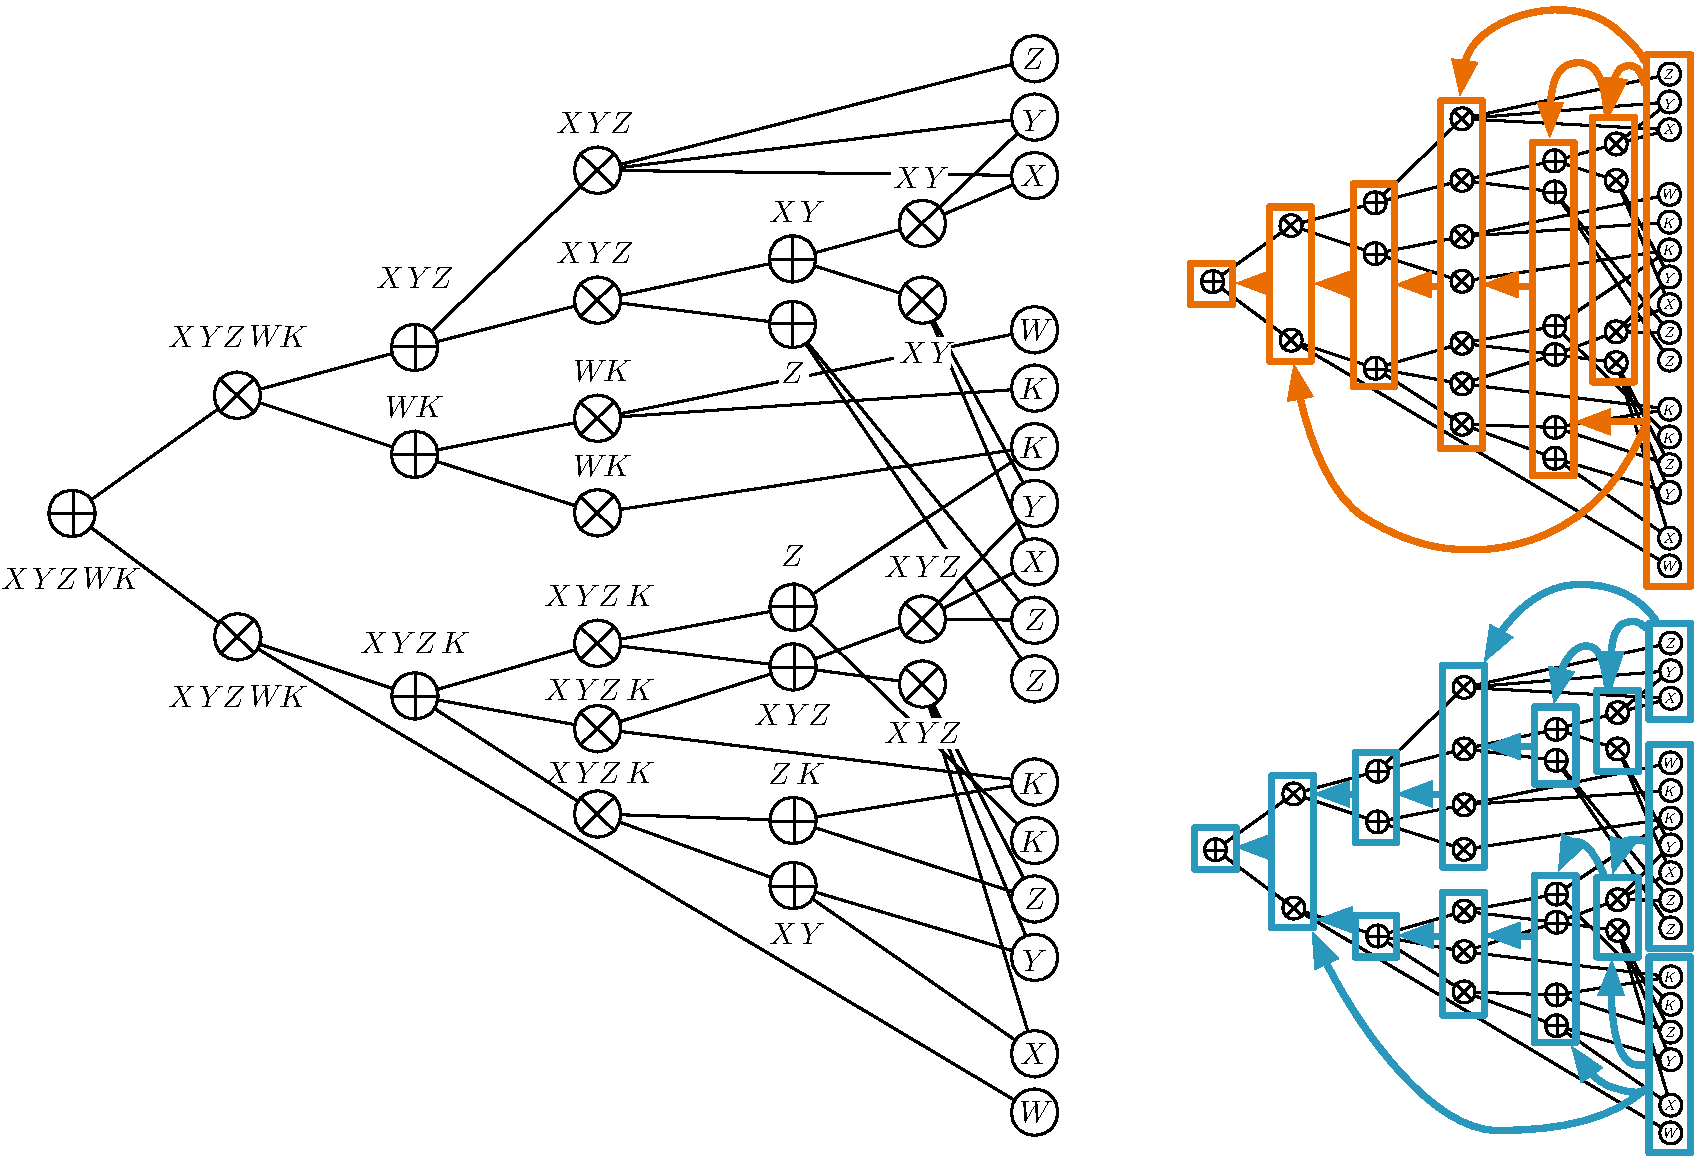
\includegraphics[width=0.8\columnwidth]{figures/layered-spn.pdf}
  \end{center}
\end{frame}

\begin{frame}
  \frametitle{SPNs as NNs (IV): filters}
  \small
  Learned features as images maximizing neuron activations\customcite{Erhan2009}:
  $$\mathbf{x}^{*} = \argmax_{\mathbf{x},
    ||\mathbf{x}||=\gamma}h_{ij}(\mathbf{x};\boldsymbol\theta).$$
  With SPNs, joint solution as an MPE assignment for all nodes (linear time):
  $$\mathbf{x}^{*}_{|\mathsf{sc}(n)} =
  \argmax_{\mathbf{x}}S_{n}(\mathbf{x}_{|\mathsf{sc}(n)};
  \mathbf{w})$$.
  \begin{center}
    \vspace{-15pt}
    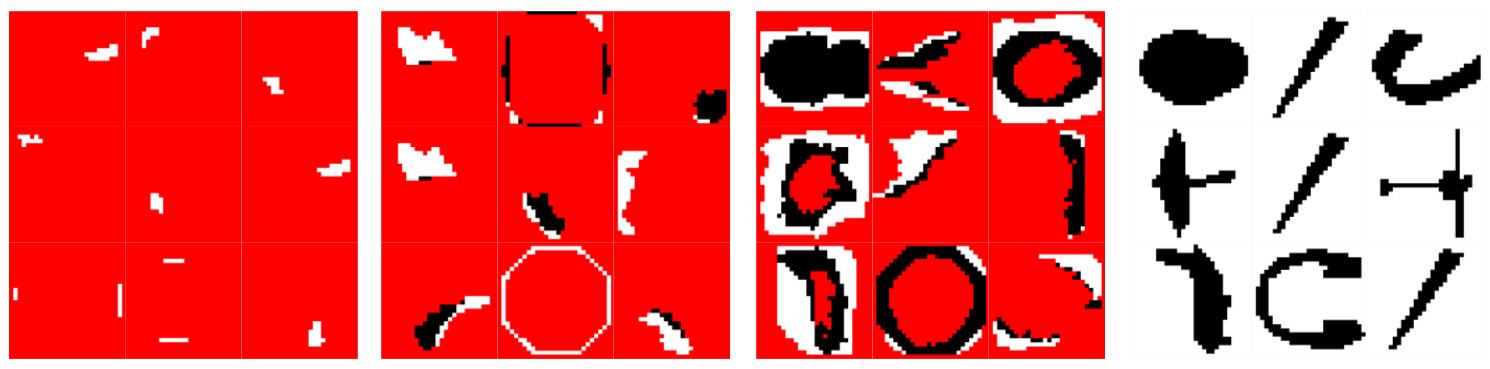
\includegraphics[width=0.9\linewidth]{figures/filters.jpg}
  \end{center}
  
  $\rightarrow$ \emph{scope length} ($|\mathsf{sc}(n)|$) correlates
  with feature abstraction level
  \customcitenomark{Vergari2016a}
\end{frame}

\begin{frame}
  \frametitle{SPNs as BNs}

Adopting Algebraic Decision Diagrams (ADDs) for  CPDs,  every  SPN  can  be  converted  into  a  BN  in  linear  time
and space  complexity  in the  size  of  the SPN
\begin{itemize}
\item the  generated  BN has  a  simple  bipartite structure
\item applying the VE algorithm to the
generated BN with ADD representation of its CPDs, the original SPN can be
recovered in linear time and space with respect to the size of the SPN
\begin{itemize}
\item the SPN can be viewed as a caching of the VE inference process
\end{itemize}
\end{itemize}
\begin{center}
  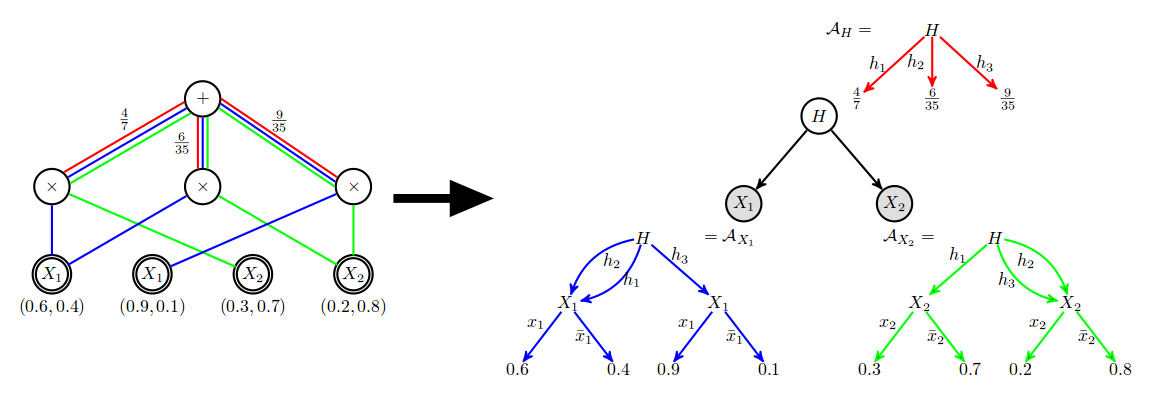
\includegraphics[width=0.7\textwidth]{figures/spn-bn}
\end{center}
  Figure from \customcite{Zhao2015}. Construct a BN with CPDs represented by ADDs from an SPN. 
\end{frame}

\section{Learning}
{\setbeamertemplate{headline}{}
  \begin{frame}[c]
    \sectionpage
  \end{frame}
}

\begin{frame}
\frametitle{Learning SPNs}
  \textbf{Parameter learning:} estimate $\mathbf{w}$ from data
  considering an SPN as a latent RV model, or as a NN.\par\bigskip

  \textbf{Structure learning:} build the network from data by assigning
  scores to tentative structures or by exploiting constraints\par\bigskip

  How to learn a ``complete'' SPN:
  \begin{itemize}
  \item handcrafted structure, then parameter learning~\parencite{Poon2011}~\parencite{Gens2012}
  \item random structures, then parameter learning~\parencite{Rashwan2016}
  \item structure learning, then parameter learning (fine tuning)~\parencite{Zhao2016a}
  \item learn both weight and structure at the same time~\parencites{Gens2013,Rooshenas2014,Vergari2015,Adel2015}~\dots  
  \end{itemize}
\end{frame}

\begin{frame}
  \frametitle{Structure Learning}

  \textbf{Score vs constraint based search.}
  No closed form for likelihood scores, need
  heuristics~\parencite{Rooshenas2014}.\par
  No need for it by exploiting the inner nodes probabilistic semantics\par\bigskip
  
  \textbf{Learning graph vs tree structures}:
  Easier to learn a tree SPN (sometimes SPT) with greedy
  approaches. Graph SPNs may be more compact and expressive efficient.\par\bigskip

  \textbf{Top-down vs bottom-up approaches}: iteratively cluster data
  matrix (top-down) or start by the marginal RVs (bottom-up)\par\bigskip

  \textbf{LearnSPN} is a \emph{\textbf{greedy}}, \emph{\textbf{top down}}, \emph{\textbf{constraint
      based}} learner for \emph{\textbf{tree}} SPNs~\parencite{Gens2013}\par
  $\rightarrow$ First principled top-down learner, inspired many algorithms and
  variations.
  $\rightarrow$ Surprisingly simple and accurate.
\end{frame}



\begin{frame}[t]
  \frametitle{LearnSPN (I)}
  Build a tree SPN by recursively split the data matrix:

  \begin{itemize}
  \item splitting columns into pairs by a greedy \textbf{\emph{G Test}} with threshold $\rho$:
    \[
      G(X_i, X_j) =  2\sum_{x_i \sim X_i}\sum_{x_j \sim X_j}c(x_i, x_j)\cdot \log\frac{c(x_i, x_j)\cdot |T|}{c(x_i)c(x_j)}
    \]
  \item clustering instances into $|C|$ sets with \textbf{\emph{online
        Hard-EM}},  estimating weights as cluster proportions with cluster penalty
    $\lambda$
    \[\begin{array}{cc}
        p(\mathbf{X})= \sum_{C_i \in \mathbf{C}}\prod_{X_j \in \mathbf{X}}p(X_j|C_i)p(C_i)\\
        % & Pr(C_i) \propto e^{-\lambda |\mathbf{C}|\cdot |\mathbf{X}|}\\
      \end{array}\]
  \item if there are less than $m$ instances, put a \textbf{\emph{naive
        factorization}} over leaves
  \item each univariate distribution get \emph{\textbf{ML estimation}} smoothed by $\alpha$  
  \end{itemize}\par\bigskip

  Hyperparameter space: $\{\rho, \lambda, m, \alpha\}$.
\end{frame}

\begin{frame}
  \frametitle{LearnSPN (II)}
  \footnotesize
  \onslide<1-4>{\begin{minipage}[t]{0.3\linewidth}
      \begin{center}
        \only<1>{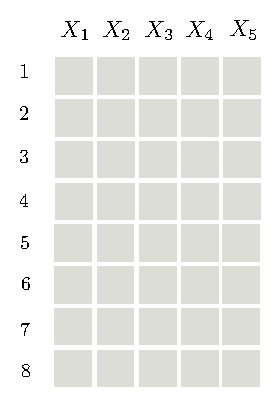
\includegraphics[width=0.8\linewidth]{figures/grid-0}}
        \only<2-4>{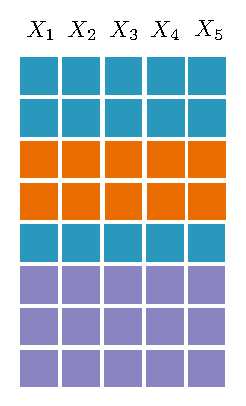
\includegraphics[width=0.715\linewidth]{figures/grid-1}}
      \end{center}
    \end{minipage}}\hspace{10pt}\onslide<3-4>{\begin{minipage}[t]{0.3\linewidth}
      \begin{center}
        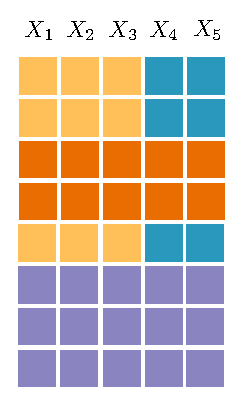
\includegraphics[width=0.72\linewidth]{figures/grid-2}
      \end{center}
    \end{minipage}}\hspace{10pt}\onslide<4>{\begin{minipage}[t]{0.3\linewidth}
      \begin{center}
        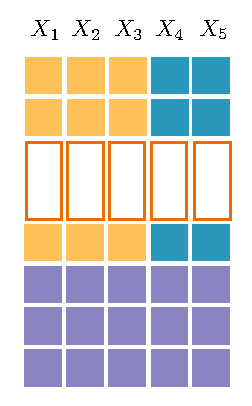
\includegraphics[width=0.735\linewidth]{figures/grid-3}
      \end{center}
    \end{minipage}}\\
  \vspace{15pt}
  \onslide<2-4>{\raisebox{0pt}{\begin{minipage}[t]{0.3\linewidth}
        \begin{center}
          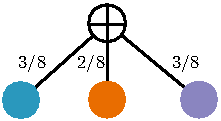
\includegraphics[width=0.715\linewidth]{figures/learnspn-1-w}
        \end{center}
      \end{minipage}}}\hspace{5pt}\onslide<3-4>{\raisebox{-25pt}{\begin{minipage}[t]{0.3\linewidth}
        \begin{center}
          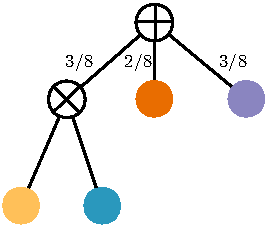
\includegraphics[width=0.83\linewidth]{figures/learnspn-2-w}
        \end{center}
      \end{minipage}}}\hspace{4pt}\onslide<4>{\raisebox{-22pt}{\begin{minipage}[t]{0.3\linewidth}
        \begin{center}
          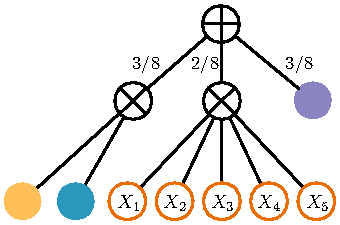
\includegraphics[width=1.0\linewidth]{figures/learnspn-3-w}
        \end{center}
      \end{minipage}}}
\end{frame}

\begin{frame}
  \frametitle{Tweaking LearnSPN}
%  \footnotesize
  
  \textsf{LearnSPN} performs two interleaved greedy
  \textbf{\emph{hierarchical divisive clustering}}
  processes (co-clutering on the data matrix).\par\bigskip

  Fast and simple. But both processes never look back and are
  committed to the choices they take \emph{\color{gold2}$\rightarrow$ slow down the two
  processes}\par\bigskip

  Online EM does not need to specify the number of clusters $k$ in
  advance. But overcomplex structures are learned by exploding the number of sum
  node children \emph{\color{gold2}$\rightarrow$ look for deeper networks}\par\bigskip

  Tractable leaf estimation. But too strong naive factorization independence
  assumptions, hard to regularize \emph{\color{gold2}$\rightarrow$ learn tree
    distributions as leaves}\par\bigskip

  ML estimations are effective. But they are not robust to noise, they
  can overfit the training set easily
  \emph{\color{gold2}$\rightarrow$ learn bagged sum nodes}
\end{frame}

\begin{frame}
  \frametitle{Why Structure Quality Matters}

  Tractable inference is guaranteed \emph{if the network size is polynomial} in $|\mathbf{X}|$.\par\bigskip

  Network \emph{\textbf{size}} influences inference complexity: smaller networks,
  faster inference!\par
  $\rightarrow$ Comparing network sizes is better than comparing inference times\par\bigskip

  Network \emph{\textbf{depth}} influences \emph{expressive efficiency}~\parencite{Martens2014}~\parencite{Zhao2015}\par\bigskip

  Structural simplicity as a bias: overcomplex networks may not generalize well.\par\bigskip
  
  Structure quality desiderata: \textbf{\textbf{smaller}} but \textbf{\textbf{accurate}}, \textbf{deeper} but not
  wider, SPNs.
\end{frame}

\begin{frame}
  \frametitle{LearnSPN-b}
  Observation: each clustering process benefits from the other one improvements/highly suffers
  from other's mistakes.\par\bigskip

  Idea: slow them down the processes by limiting the number of
  nodes to split to the minimum.
  \textsf{LearnSPN-b}, binary splitting $k=2$.\par%\bigskip

  $\rightarrow$ one hyperparameter less, $\lambda$.\par%\bigskip
  $\rightarrow$ not committing to complex structures too early\par
  $\rightarrow$ reducing node out fan increases the depth\par
  $\rightarrow$ same expressive power as LearnSPN structures\par
  $\rightarrow$ statistically same (or better) accuracy, smaller
  networks\par%\bigskip
  \begin{center}
    \raisebox{19pt}{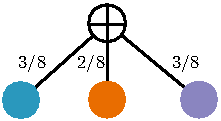
\includegraphics[width=0.23\linewidth]{figures/learnspn-1-w.pdf}}
    \raisebox{30pt}{\hspace{20pt}\Huge$=$\hspace{10pt}}
    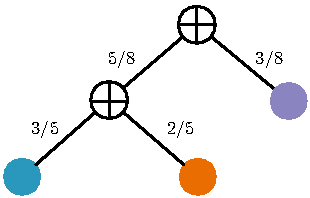
\includegraphics[width=0.3\linewidth]{figures/learnspn-4-w.pdf}
  \end{center}

  % \raisebox{45pt}{\begin{minipage}[t]{0.65\linewidth}
%       Objectives:
%       \begin{itemize}
%       \item not committing to complex structures too early
%       \item same expressive power as LearnSPN
%       \item reducing node out fan increases the depth
%       \item statistically same (or better) accuracy, smaller networks
%       \end{itemize}
%     \end{minipage}}\hspace{-5pt}\begin{minipage}[t]{0.3\linewidth}
%     \begin{center}
%       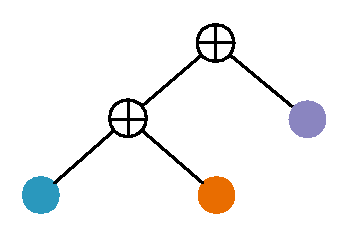
\includegraphics[width=0.9\linewidth]{figures/learnspn-4.pdf}
%     \end{center}
%   \end{minipage}\footfullcitenomark{Vergari2015}
%
  \end{frame}

\begin{frame}
  \frametitle{LearnSPN-b: depth VS size}
  \begin{figure}[htbp]
    \begin{center}
      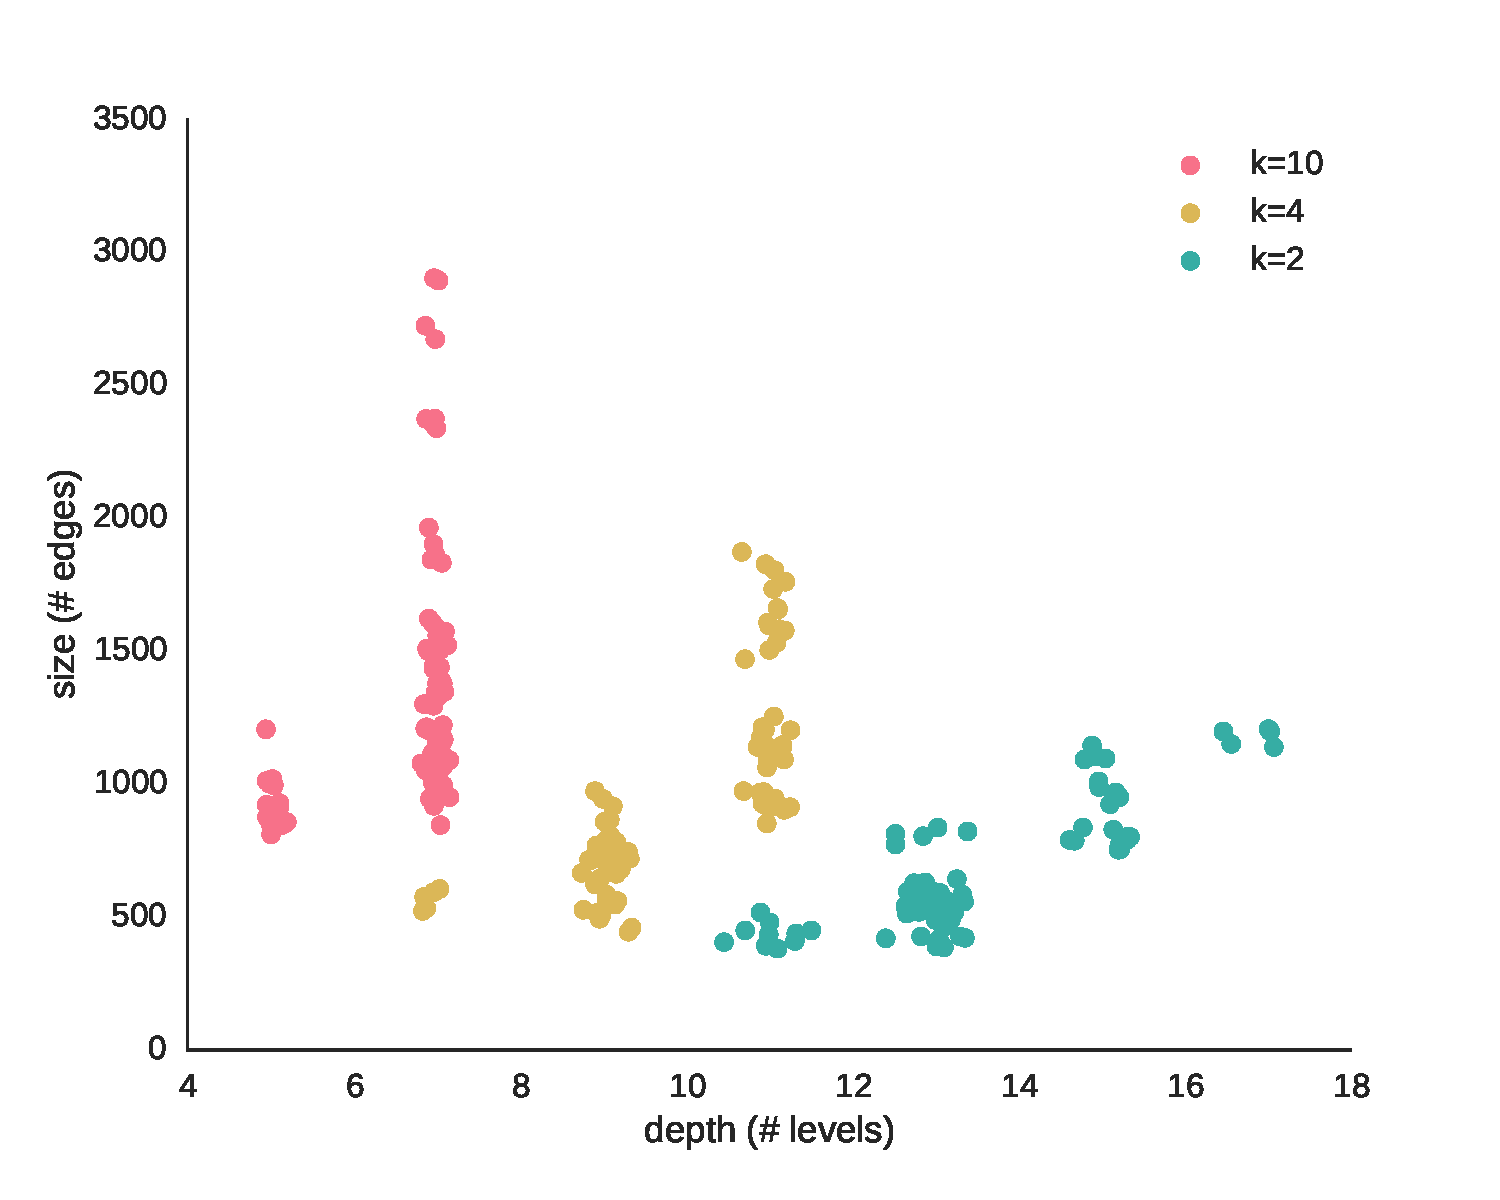
\includegraphics[width=0.5\linewidth]{figures/nltcs-depth.pdf}
      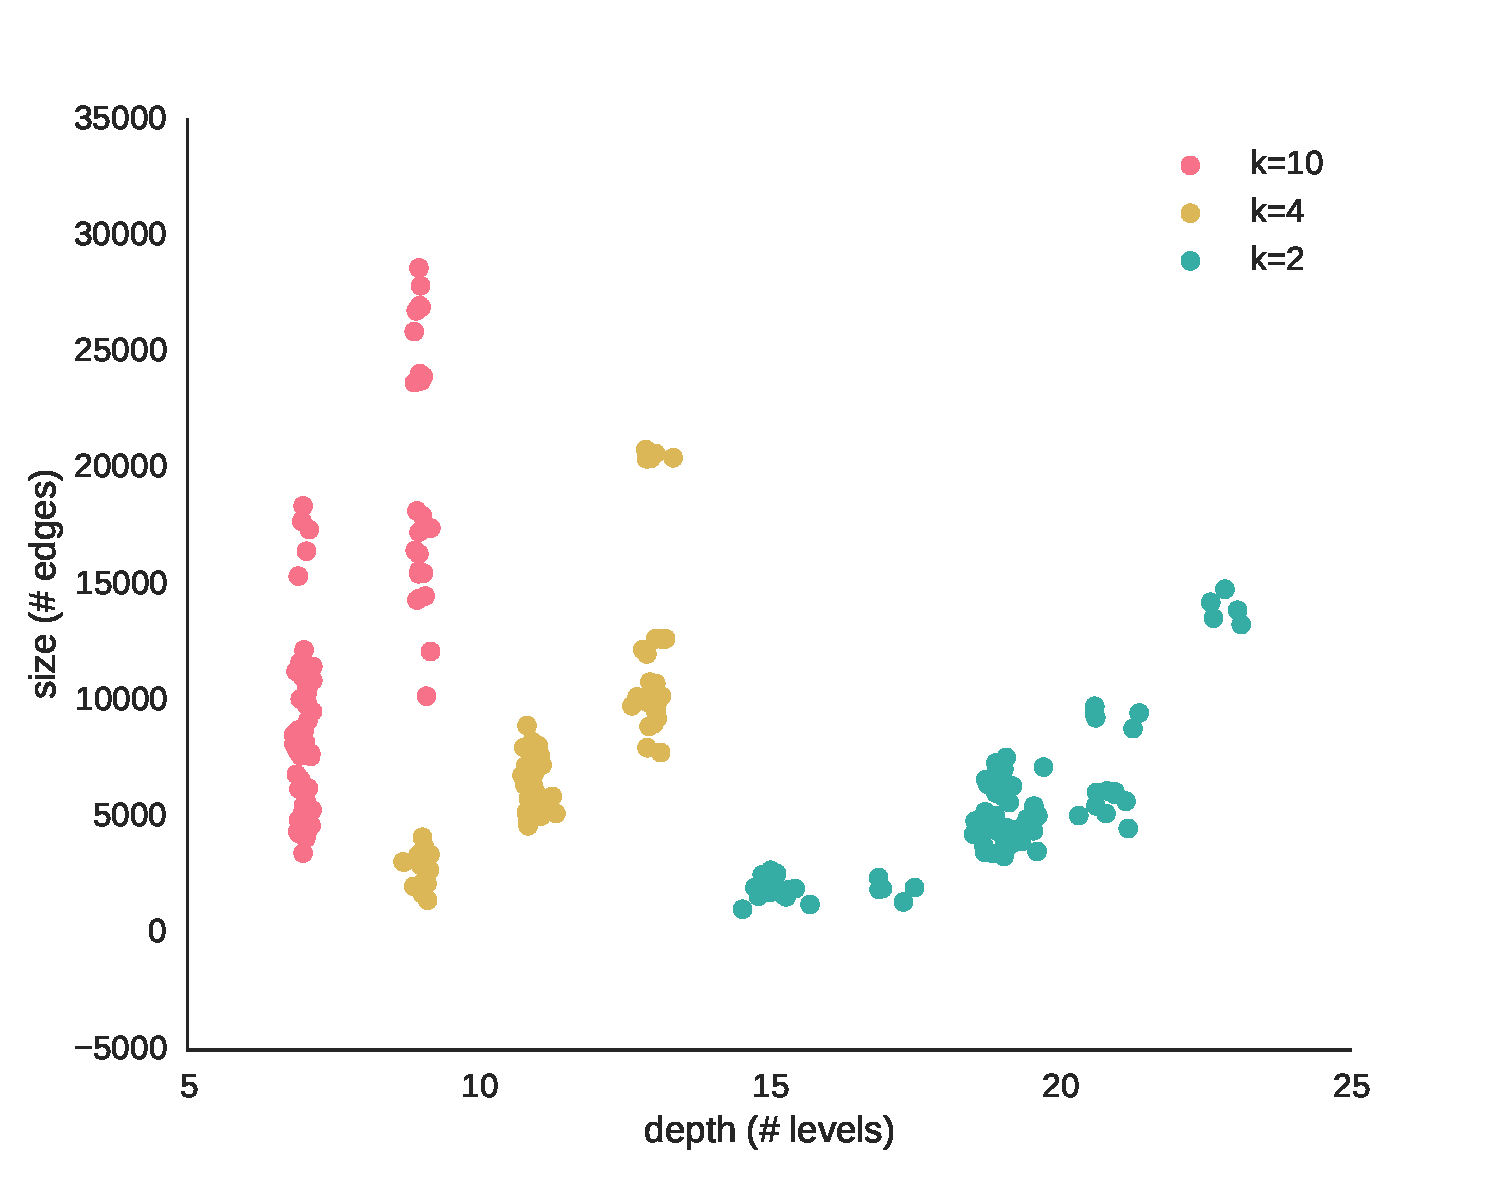
\includegraphics[width=0.5\linewidth]{figures/plants-depth.pdf}
      \caption{\footnotesize
        Network sizes VS depths while varying the max
        number of sum node children splits ($k\in\{10, 4, 2\}$). Each dot is an experiment
        in the grid search hyperparameter space performed by
        \textsf{LearnSPN-b} on NLTCS (left) and Plants (right).}
    \end{center}
  \end{figure}
\end{frame}

\begin{frame}
  \frametitle{LearnSPN-b: best ll VS size}

  \begin{figure}[htbp]
    \begin{center}
      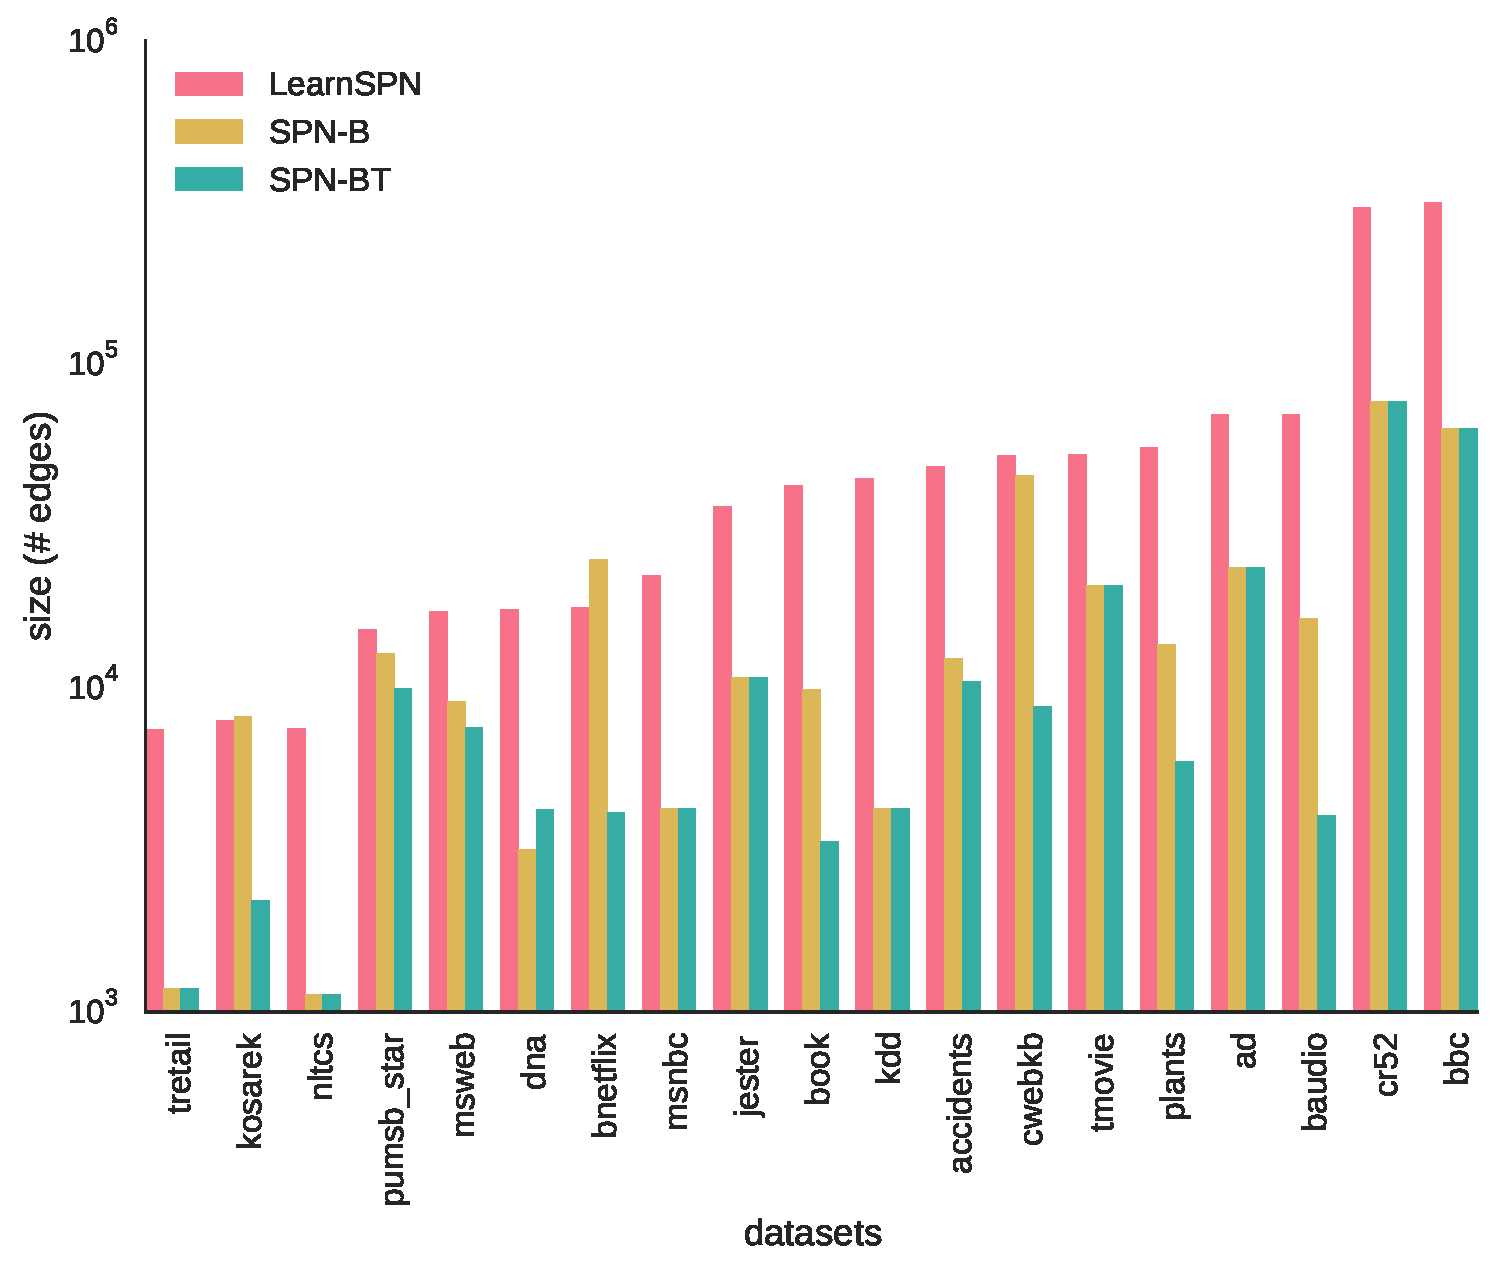
\includegraphics[width=0.65\linewidth]{figures/edges-comp.pdf}
      \caption{\footnotesize
        Comparing network sizes
        for the networks scoring the best log-likelihoods in the grid
        search as obtained by \textsf{LearnSPN}, \textsf{LearnSPN-b} and
        \textsf{LearnSPN-bT} for each dataset.}
    \end{center}
  \end{figure}
\end{frame}

\begin{frame}
  \frametitle{Other variations on LearnSPN}
  \textbf{ACs modeling leaves} by performing a greedy score
  search.
  \emph{\textbf{ID-SPN}} best log-likelihood learner (but lots of
  hyperparameters).\par
  Freely available in the \textsf{Libra}\footnote{http://libra.cs.uoregon.edu/} toolkit~\parencite{Rooshenas2014}\par\bigskip
  
  Looking for \textbf{correlations instead of independencies} via matrix
  factorizations.\par
  Splitting matrix rows and columns at the same time: SPN-SVD.\par
  It can cope with continuous data~\parencite{Adel2015}\par\bigskip
  
  Post-learning \textbf{mergining sub-SPNs} that model ``similar'' distributions.\par
  Reducing network sizes~\parencite{Rahman2016}.\par\bigskip

  Learning Relational SPNs on \textbf{first order data}
  represented in Tractable Markov Logic (TML), \emph{LearnRSPN}~\parencite{Nath2015}.
\end{frame}

\begin{frame}
  \frametitle{Other Tendencies in Structure Learning}
  \textbf{Learning deterministic structures} which enable closed form
  log-likelihood and weight estimation.\par
  Selective SPNs, enabling efficient Stochastic Local
  Search~\parencite{Peharz2014b}.\par
  Mixing latent and deterministic mixtures as sum
  nodes (a Cutset Network is an
  SPN!)~\parencite{Rahman2016}\par\bigskip
  
  \textbf{Learning DAGs} structures instead of trees.\par
  Substituting sub-structures with more complex ones by cloning mixtures~\parencite{Dennis2015}\par\bigskip
  
  \textbf{Template learning} for sequence
  models.
  Stochastic local search over well defined constrained structures.
  Dynamic SPNs~\parencite{Melibari2016c}\color{gold2}\emph{$\rightarrow$ PGM'16!}\par\bigskip
\end{frame}

\begin{frame}
  \frametitle{Parameter Learning}
  Non convex optimization, solvable with (online) iterative methods
  (e.g. SGD)\par\bigskip

  Classical approach: compute the gradient $\nabla_{\mathbf{w}}
  S(\mathbf{x})$\par
  $\rightarrow$ use backpropagation (differential
  approach\customcite{Darwiche2003})\par
  \begin{enumerate}
  \item $\nabla_{S(\mathbf{x})} S(\mathbf{x})\leftarrow 1$ start from
    the root
  \item if $n$ is a sum node, $\forall_{c\in\mathsf{ch}(n)}$:\par
    $\nabla_{S_{c}(\mathbf{x})}S(\mathbf{x})\leftarrow
    \nabla_{S_{c}(\mathbf{x})}S(\mathbf{x}) + w_{nc}\nabla_{S_{n}(\mathbf{x})}S(\mathbf{x})$ 
  \item if $n$ is a product node, $\forall_{c\in\mathsf{ch}(n)}$:\par
    $\nabla_{S_{c}(\mathbf{x})}S(\mathbf{x})\leftarrow
    \nabla_{S_{c}(\mathbf{x})}S(\mathbf{x}) + \nabla_{S_{n}(\mathbf{x})}S(\mathbf{x})\prod_{k\in\mathsf{ch}(n)\setminus\{c\}}S_{k}(\mathbf{x})$
  \end{enumerate}
  \par%\bigskip

  %Hard/Soft gradients\par\bigskip

  Issues:
  \begin{itemize}
  \item vanishing gradients: depth is a major problem for \emph{soft} gradients
  \item hyperparameter choices
    \begin{itemize}
    \item adaptive learning rate scheduling algos not employed yet!
    \end{itemize}
  \end{itemize}
\end{frame}

\begin{frame}
  \frametitle{``Hard'' gradients}
  \begin{minipage}{0.4\linewidth}
    \vspace{10pt}
    \begin{center}
      \only<1>{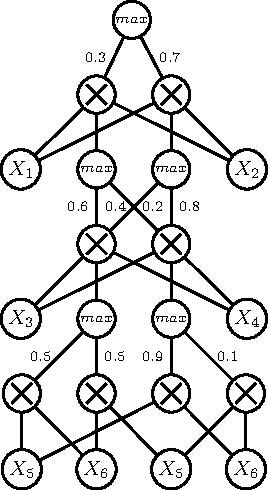
\includegraphics[width=0.75\columnwidth]{figures/spn-eval-mpe-1}}
      \only<2>{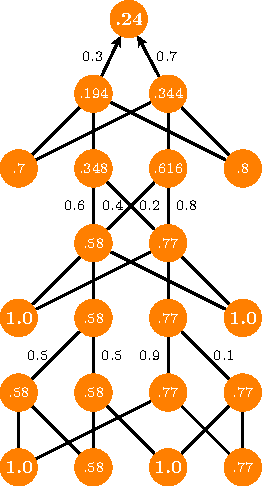
\includegraphics[width=0.75\columnwidth]{figures/spn-eval-mpe-2}}
      \only<3-4>{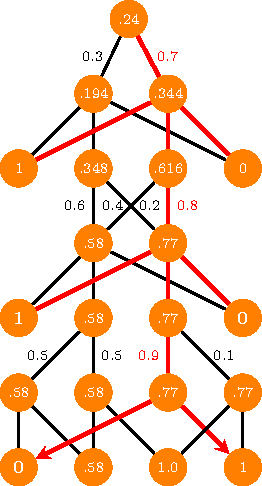
\includegraphics[width=0.75\columnwidth]{figures/spn-eval-mpe-5}}
    \end{center}
  \end{minipage}\hfill\begin{minipage}[t]{0.58\linewidth}
    \vspace{-80pt}
    From SPN $S$ to MPN $M$\par
    \begin{itemize}
    \item<2-4> forward (bottom-up) prop $\mathbf{x}^{i}$
    \item<3-4> backprop as MPE descent
    \item<4> ``count'' the \colorbox{red}{\textcolor{white}{weights}}
      occurrencies in the path $W_{\mathbf{x}^{i}}$
      $$\nabla_{w_{pc}}
      \log M(\mathbf{x})=\frac{\sharp\{w_{pc}\in W_{\mathbf{x}}\}}{w_{pc}}$$
    \end{itemize}
    \only<4>{
      \hspace{15pt}$\rightarrow$ not vanishing (regardless depth)\par
      \hspace{15pt}$\rightarrow$ slower convergence\par\hspace{27pt}(less updates/instance)}
    
  \end{minipage}
  \customcitenomark{Poon2011}
  \customcitenomark{Gens2012}
\end{frame}

\begin{frame}
  \frametitle{Hard/Soft Parameter Updating}
  \begin{table}
    \centering
    \begin{tabular}{l c}
      & $\Delta w_{pc}$\\
      \toprule
      \textsf{\textbf{Soft Gradient}}&\\
      \textsf{\emph{Generative}} ($\nabla_{w_{pc}}
      S(\mathbf{x})$) & $ S_{c}(\mathbf{x})\nabla_{S_{p}(\mathbf{x})}
                         S(\mathbf{x})$\\
      \textsf{\emph{Discriminative}} ($\nabla_{w_{pc}}\log
      S(\mathbf{y}|\mathbf{x})$) &
                                   $\frac{\nabla_{w_{pc}}S(\mathbf{y}|\mathbf{x})}{S(\mathbf{y}|\mathbf{x})}  - \frac{\nabla_{w_{pc}}S(\mathbf{*}|\mathbf{x})}{S(\mathbf{*}|\mathbf{x})}$\\
      \textsf{\textbf{Hard Gradient}}& \\
      \textsf{\emph{Generative}} ($\nabla_{w_{pc}}
      \log M(\mathbf{x})$)                   &
                      % $\frac{\sharp\{w_{pc}\in
                      % \mathsf{MPE-path}(\mathbf{x})\}}{w_{pc}}$\\
      $\frac{\sharp\{w_{pc}\in W_{\mathbf{x}}\}}{w_{pc}}$\\
      \textsf{\emph{Discriminative}}
      ($\nabla_{w_{pc}}\log
      M(\mathbf{y}|\mathbf{x})$)
                      &
                                                    $\frac{\sharp\{w_{pc}\in
                        W_{(\mathbf{y}|\mathbf{x})}\}
                                                    - \sharp\sharp\{w_{pc}\in
                        W_{(\mathbf{1}|\mathbf{x})}\}}{w_{pc}}$\\
      \midrule
      \textsf{\textbf{Soft} Posterior}\customcite{Peharz2016} ($p(H_{p}=c|\mathbf{x})$) & $\propto \frac{1}{S(\mathbf{x})}\frac{\partial
                                      S(\mathbf{x})}{\partial
                                                                  S_{p}(\mathbf{x})}S_{c}(\mathbf{x})w_{pc}$ \\
      \textsf{\textbf{Hard} Posterior} ($p(H_{p}=c|\mathbf{x})$) & $=
                                                                                             \begin{cases}
                                                                                               1
                                                                                               \text{if}
                                                                                               w_{pc}
                                                                                               \in W_{\mathbf{x}}
                                                                                               \\
                                                                                               0 \text{otherwise}
                                                                                             \end{cases}
$\\
    \end{tabular}
  \end{table}
  \customcitenomark{Gens2012}
\end{frame}

\begin{frame}
  \frametitle{Bayesian Parameter Learning}
  Learning in a Bayesian setting is computing the posterior $p(\mathbf{w}|\{\mathbf{x}^{i}\}_{i=1}^{m})$ having
  a prior $p(\mathbf{w})$:
  % p(\mathbf{w}|\{\mathbf{x}^{i}\}_{i=1}^{m})\propto p(\mathbf{w})p(\{\mathbf{x}^{i}\}_{i=1}^{m}|\mathbf{w})\par
  $$p(\mathbf{w}|\{\mathbf{x}^{i}\}_{i=1}^{t+1})\propto
  p(\mathbf{w}|\{\mathbf{x}^{i}\}_{i=1}^{t})p(\mathbf{x}^{t+1}|\mathbf{w})$$
  $p(\mathbf{w})$ modeled as a product of Dirichlet,
  $p(\mathbf{x}^{t+1}|\mathbf{w})$ is an exponential sum of monomials, $\rightarrow$ the posterior
  becomes a mixture of products of Dirichlets growing exponentially in
  the data and sum nodes!\par\bigskip

  \textbf{Online Bayesian Moment Matching} (OBMM): computing first two
  moments to approximate the intractable posterior, efficiently for
  tree SPNs~\parencite{Rashwan2016}.\par\bigskip

  \textbf{Collapse Variational Inference} (CVB-SPN) to optimize a
  logarithmic lower bound (better than ELBO) efficiently (linear in $|S|$)~\parencite{Zhao2016a}.
  
\end{frame}

\begin{frame}[t]
  \frametitle{Parameter learning}
  \vspace{-10pt}
  \begin{table}
    \centering
    \scriptsize
    \setlength{\tabcolsep}{3pt}  
    \begin{tabular}{l r r r r r}
      \toprule
      & \textsf{CVB-SPN}\customcite{Zhao2016a} &
                                                 \textsf{OBMM}\customcite{Rashwan2016} & \textsf{SGD}\footnotemark[48] & \textsf{EM}\footnotemark[48] & \textsf{SEG}\footnotemark[48] \\
      \midrule
      \textbf{NLTCS}      & -6.08   & -6.07   & -8.76   & -6.31   & -6.85   \\
      \textbf{MSNBC}      & -6.29   & -6.03   & -6.81   & -6.64   & -6.74   \\
      \textbf{KDDCup2k}   & -2.14   & -2.14   & -44.53  & -2.20   & -2.34   \\
      \textbf{Plants}     & -12.86  & -15.14  & -21.50  & -17.68  & -33.47  \\
      \textbf{Audio}      & -40.36  & -40.70  & -49.35  & -42.55  & -46.31  \\
      \textbf{Jester}     & -54.26  & -53.86  & 63.89   & -54.26  & -59.48  \\
      \textbf{Netflix}    & -60.69  & -57.99  & 64.27   & -59.35  & -64.48  \\
      \textbf{Accidents}  & -29.55  & -42.66  & 53.69   & -43.54  & -45.59  \\
      \textbf{Retail}     & -10.91  & -11.42  & -97.11  & -11.42  & -14.94  \\
      \textbf{Pumsb-star} & -25.93  & -45.27  & -128.48 & -46.54  & -51.84  \\
      \textbf{DNA}        & -86.73  & -99.61  & -100.70 & -100.10 & -105.25 \\
      \textbf{Kosarek}    & -10.70  & -11.22  & 34.64   & -11.87  & -17.71  \\
      \textbf{MSWeb}      & -9.89   & -11.33  & -59.63  & -11.36  & -20.69  \\
      \textbf{Book}       & -34.44  & -35.55  & -249.28 & -36.13  & -42.95  \\
      \textbf{EachMovie}  & -52.63  & -59.50  & -227.05 & -64.76  & -84.82  \\
      \textbf{WebKB}      & -161.46 & -165.57 & -338.01 & -169.64 & -179.34 \\
      \textbf{Reuters-52} & -85.45  & -108.01 & -407.96 & -108.10 & -108.42 \\
      \textbf{20-Newsgrp} & -155.61 & -158.01 & -312.12 & -160.41 & -167.89 \\
      \textbf{BBC}        & -251.23 & -275.43 & -462.96 & -274.82 & -276.97 \\
      \textbf{Ad}         & -19.00  & -63.81  & -638.43 & -63.83  & -64.11  \\
    \end{tabular}
    \label{tab:model-accs}
  \end{table}

\end{frame}

\begin{frame}[t]
  \frametitle{Parameter learning VS LearnSPN}
  \vspace{-10pt}
  \begin{table}
    \centering
    \scriptsize
    \setlength{\tabcolsep}{3pt}  
    \begin{tabular}{l r r r r r r r}
      \toprule
      & \textsf{LearnSPN}\customcite{Gens2013} &
                                                 \textsf{LearnSPN-b}\customcite{Vergari2015} & \textsf{CVB-SPN}\customcite{Zhao2016a} & \textsf{OBMM}\customcite{Rashwan2016} & \textsf{SGD}\footnotemark[52] & \textsf{EM}\footnotemark[52] & \textsf{SEG}\footnotemark[52] \\
      \midrule
      \textbf{NLTCS}      & -6.11   & -6.05   & -6.08   & -6.07   & -8.76   & -6.31   & -6.85   \\
      \textbf{MSNBC}      & -6.11   & -6.04   & -6.29   & -6.03   & -6.81   & -6.64   & -6.74   \\
      \textbf{KDDCup2k}   & -2.18   & -2.14   & -2.14   & -2.14   & -44.53  & -2.20   & -2.34   \\
      \textbf{Plants}     & -12.98  & -12.81  & -12.86  & -15.14  & -21.50  & -17.68  & -33.47  \\
      \textbf{Audio}      & -40.50  & -40.57  & -40.36  & -40.70  & -49.35  & -42.55  & -46.31  \\
      \textbf{Jester}     & -53.48  & -53.53  & -54.26  & -53.86  & 63.89   & -54.26  & -59.48  \\
      \textbf{Netflix}    & -57.33  & -57.73  & -60.69  & -57.99  & 64.27   & -59.35  & -64.48  \\
      \textbf{Accidents}  & -30.04  & -29.34  & -29.55  & -42.66  & 53.69   & -43.54  & -45.59  \\
      \textbf{Retail}     & -11.04  & -10.94  & -10.91  & -11.42  & -97.11  & -11.42  & -14.94  \\
      \textbf{Pumsb-star} & -24.78  & -23.31  & -25.93  & -45.27  & -128.48 & -46.54  & -51.84  \\
      \textbf{DNA}        & -82.52  & -81.91  & -86.73  & -99.61  & -100.70 & -100.10 & -105.25 \\
      \textbf{Kosarek}    & -10.99  & -10.72  & -10.70  & -11.22  & 34.64   & -11.87  & -17.71  \\
      \textbf{MSWeb}      & -10.25  & -9.83   & -9.89   & -11.33  & -59.63  & -11.36  & -20.69  \\
      \textbf{Book}       & -35.89  & -34.30  & -34.44  & -35.55  & -249.28 & -36.13  & -42.95  \\
      \textbf{EachMovie}  & -52.49  & -51.36  & -52.63  & -59.50  & -227.05 & -64.76  & -84.82  \\
      \textbf{WebKB}      & -158.20 & -154.28 & -161.46 & -165.57 & -338.01 & -169.64 & -179.34 \\
      \textbf{Reuters-52} & -85.07  & -83.34  & -85.45  & -108.01 & -407.96 & -108.10 & -108.42 \\
      \textbf{20-Newsgrp} & -155.93 & -152.85 & -155.61 & -158.01 & -312.12 & -160.41 & -167.89 \\
%      \textbf{BBC}        & -250.69 & -247.30 & -251.23 & -275.43 & -462.96 & -274.82 & -276.97 \\
%      \textbf{Ad}         & -19.73  & -16.23  & -19.00  & -63.81  & -638.43 & -63.83  & -64.11  \\
    \end{tabular}
    \label{tab:model-accs}
  \end{table}
\end{frame}


\begin{frame}
  \frametitle{Why learning parameters only}
  Even if simple, \textsf{LearnSPN} hardly scales on large datasets.\par
  $\rightarrow$ generate a random (but valid) structure, then optimize the weights
  \begin{table}
    \centering
    \scriptsize
    \setlength{\tabcolsep}{3pt}  
    \begin{tabular}{l r r r r r r}
      \toprule
      & \textsf{LearnSPN}& \textsf{OBMM} & \textsf{ODMM} & \textsf{SGB} & \textsf{OEM} & \textsf{OEG} \\
      \midrule
      \textbf{KOS} & -444.55 & \textbf{-422.19} & -437.30 & -3492.9 & -538.21 & -657.13\\
      \textbf{NIPS} & - &  \textbf{-1691.87}& -1709.04& -7411.20& -1756.06 & -3134.59 \\
      \textbf{ENRON} & - &\textbf{-518.842}& -522.45& -13961.40& -554.97 & -14193.90\\
      \textbf{NyTIMES} & - & -1503.65& -1559.39& -43153.60& \textbf{-1189.39} & -6318.71\\
      \bottomrule
    \end{tabular}
    \label{tab:model-accs}
  \end{table}

  $\rightarrow$ distribute the computation of gradients and updates
  (over instances,\dots etc)
  \begin{table}
    \centering
    \scriptsize
    \setlength{\tabcolsep}{3pt}  
    \begin{tabular}{l r r r r r r}
      \toprule
      & \textsf{LearnSPN}& \textsf{OBMM} & \textsf{ODMM} & \textsf{SGB} & \textsf{OEM} & \textsf{OEG} \\
      \midrule
      \textbf{KOS} & 1439.11 & 89.40 & \textbf{8.66} & 162.98 & 59.49 & 155.34\\
      \textbf{NIPS} & - &  139.50& \textbf{9.43}& 180.25& 64.62 & 178.35 \\
      \textbf{ENRON} & - &2018.05& \textbf{580.63}& 876.18& 694.17 & 883.12\\
      \textbf{NyTIMES} & - & 12091.7& \textbf{1643.60}& 5626.33& 5540.40 & 6895.00\\
      \bottomrule
    \end{tabular}
    \label{tab:model-accs}
  \end{table}
  \customcitenomark{Rashwan2016}
\end{frame}

\begin{frame}
  \frametitle{Other Tendencies in Parameter Learning}
  \textbf{Jointly learning leaf distributions} parameters while optimizing.\par
  E.g. deriving EM update rules for leaf distributions~\parencites{Peharz2015,Desana2016}\par\bigskip
  
   \textbf{Bayesian learning with continous leaf}
  distributions. Extending OBMM to tree SPNs with continuous Gaussian
  leaves~\parencite{Jaini2016}{\color{gold2}\emph{$\rightarrow$
    PGM'16!}}\par\bigskip

  Non bayesian \textbf{signomial programming approaches} still
  considering an SPN as a (very large)
  mixture over tree distributions.\par
  Multiplicative updates (no projections, like EG, but faster convergence) for Sequential
  Monomial Approximations (SMA) and Concave-Convex procedure (CCCP)~\parencite{Zhao2016b}\par\bigskip
\end{frame}


\section{Applications}
{\setbeamertemplate{headline}{}
  \begin{frame}[c]
    \sectionpage
  \end{frame}
}

\begin{frame}
  \frametitle{Applications I: computer vision}
  
\end{frame}


\begin{frame}
  \frametitle{Applications II: language modeling}
  
\end{frame}

\begin{frame}
  \frametitle{Applications III: activity recognition}
\end{frame}

\begin{frame}
  \frametitle{Applications IV: speech}
  SPNs to model the joint pdf of observed RVs in HMMs (HMM-SPNs).
  \begin{center}
    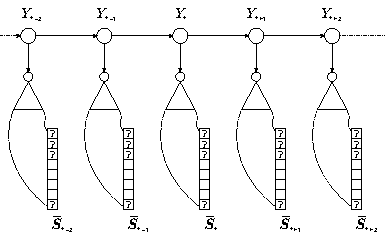
\includegraphics[width=0.35\columnwidth]{figures/peharz2014a-figures/hmm-spn-model}
  \end{center}\par

  State-of-the-art high frequency reconstruction (MPE inference)
  \begin{center}
    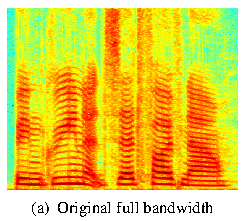
\includegraphics[width=0.25\columnwidth]{figures/peharz2014a-figures/orig}
    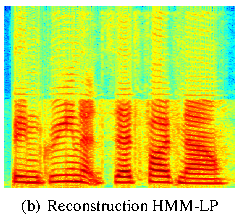
\includegraphics[width=0.25\columnwidth]{figures/peharz2014a-figures/hmm-lp}
    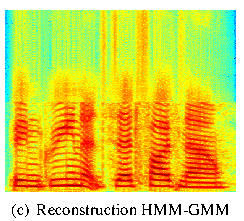
\includegraphics[width=0.25\columnwidth]{figures/peharz2014a-figures/hmm-gmm}
    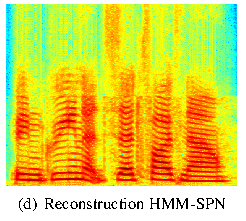
\includegraphics[width=0.25\columnwidth]{figures/peharz2014a-figures/hmm-spn}
  \end{center}
  
  \customcitenomark{Peharz2014a}
\end{frame}


\section{Representation Learning}
{\setbeamertemplate{headline}{}
  \begin{frame}[c]
    \sectionpage
  \end{frame}
}

\begin{frame}
  \frametitle{Extracting Embeddings}
  \framesubtitle{From deep neural networks}
  \begin{minipage}{0.38\linewidth}
    \begin{center}
      \only<1>{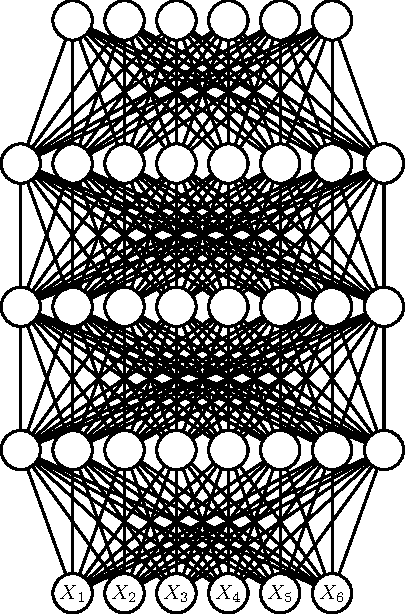
\includegraphics[width=.9\columnwidth]{figures/dnn-eval-emb-I}}
      \only<2>{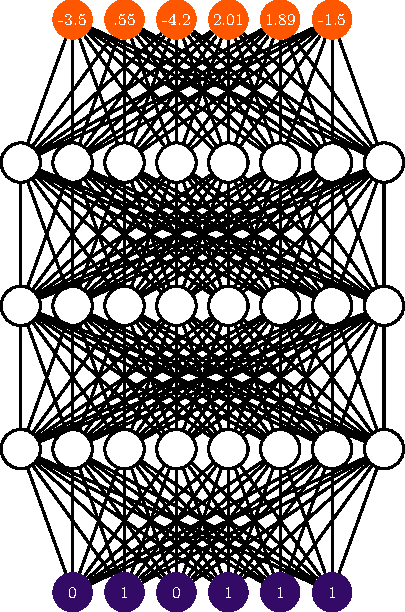
\includegraphics[width=.9\columnwidth]{figures/dnn-eval-emb-II}}
    \end{center}
  \end{minipage}\hfill\begin{minipage}[t]{0.6\linewidth}
    \vspace{-80pt}
    Build an embedding $\mathbf{e}^{i}\in\mathbb{R}^{d}$ for sample
    $$\mathbf{x}^{i}=\langle 0,1,0,1,1,1 \rangle$$
    \only<2>{by evaluating the network and collecting the last layer(s) activations
      \scriptsize\begin{align*}
                   \mathbf{e}^{i}= \langle&\highlight[lacamgold5]{-3.5},\highlight[lacamgold5]{.55},\highlight[lacamgold5]{-4.2},\highlight[lacamgold5]{2.01},\highlight[lacamgold5]{1.89},\highlight[lacamgold5]{-1.5}\rangle
      \end{align*}}

  \end{minipage}
  \customcitenomark{Bengio2012}
\end{frame}

\begin{frame}
  \frametitle{Extracting Embeddings}
  \framesubtitle{Exploiting SPNs as feature extractors  }

  Given an SPN $S$, a filtering criterion $f$, generate a dense vector
  for each sample $\mathbf{x}^{i}$
  $$\mathbf{e}^{i} =f_{S}(\mathbf{x}^{i})$$
  
  Issues with SPNs as NNs:
  \begin{itemize}
  \item layer-wise extraction may be arbitrary
  \item power law distribution of nodes by scopes
    \item scope lengths as proxy for feature abstraction levels (see filter visualizations)
    \end{itemize}

    Which filtering criterion to employ?\par
    Which interpretation for the extracted features?
  
  
  % How to extract embeddings?
  % \begin{itemize}
  % \item from node outputs (one query) 
  %   \begin{itemize}
  %   \item all (non-leaf) nodes
  %   \item sum/product nodes only
  %   \item with a certain scope length
  %     \item aggregating node outputs by scope
  %   \end{itemize}
  % \item from several queries evaluations (root outputs)
  % \end{itemize}
  \customcitenomark{Vergari2016a}
\end{frame}

\begin{frame}
  \frametitle{Extracting embeddings}
  \framesubtitle{Inner node activations}
  \begin{minipage}{0.4\linewidth}
    \begin{center}
      \only<1>{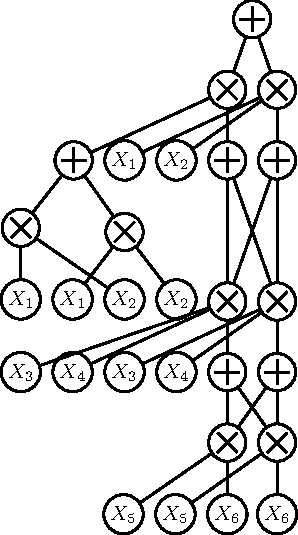
\includegraphics[width=.85\columnwidth]{figures/spn-emb}}
      \only<2>{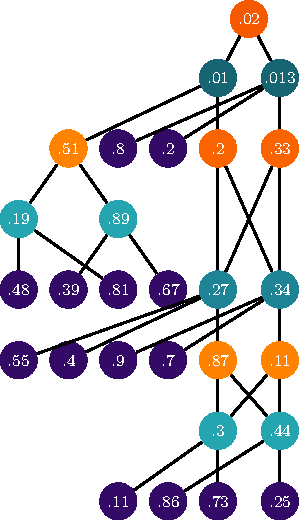
\includegraphics[width=.86\columnwidth]{figures/spn-emb-eval}}
    \end{center}
  \end{minipage}\hfill\begin{minipage}[t]{0.55\linewidth}
    \vspace{-80pt}
    Build an embedding $\mathbf{e}^{i}\in\mathbb{R}^{d}$ for sample
    $$\mathbf{x}^{i}=\langle 0,1,0,1,1,1 \rangle$$
    \only<2>{by evaluating $S(\mathbf{x}^{i})$ and collecting inner node
    (\colorbox{gold4}{\textcolor{white}{sum}}, \colorbox{petroil4}{\textcolor{white}{product}} but not 
    \colorbox{lacamdarklilac5}{\textcolor{white}{leaves}}) activations
    \scriptsize
    \begin{align*}
    \mathbf{e}^{i}= \langle&\highlight[gold6]{.02},\highlight[petroil6]{.01},\highlight[petroil6]{.013},\highlight[gold2]{.51},\highlight[gold4]{.2},\highlight[gold4]{.33},\\
                   &\highlight[petroil2]{.19},\highlight[petroil2]{.89},\highlight[petroil4]{.27},\highlight[petroil4]{.34},\highlight[gold2]{.87},\highlight[gold2]{.11},\\
      &\highlight[petroil2]{.3},\highlight[petroil2]{.44}  \rangle
  \end{align*}}

  \end{minipage}
\end{frame}

\begin{frame}
  \frametitle{Extracting embeddings}
  \framesubtitle{Filtering by type}
  \begin{minipage}{0.4\linewidth}
    \begin{center}
      \includegraphics[width=.86\columnwidth]{figures/spn-emb-eval}
    \end{center}
  \end{minipage}\hfill\begin{minipage}[t]{0.55\linewidth}
    \vspace{-80pt}
    Build embeddings $\mathbf{e}^{i}_{\mathsf{sum}}, \mathbf{e}^{i}_{\mathsf{prod}}$ for sample
    $$\mathbf{x}^{i}=\langle 0,1,0,1,1,1 \rangle$$
    by evaluating $S(\mathbf{x}^{i})$ and collecting
    inner node activations filtered by node type
    \scriptsize
      \begin{align*}
        \mathbf{e}^{i}_{\mathsf{sum}}= \langle&\highlight[gold6]{.02},\highlight[gold2]{.51},\highlight[gold4]{.2},\highlight[gold4]{.33},\highlight[gold2]{.87},\highlight[gold2]{.11} \rangle\\
        \mathbf{e}^{i}_{\mathsf{prod}}=\langle&\highlight[petroil6]{.01},\highlight[petroil6]{.013},\highlight[petroil2]{.19},\highlight[petroil2]{.89},\highlight[petroil4]{.27},\highlight[petroil4]{.34},\\
        &\highlight[petroil2]{.3},\highlight[petroil2]{.44}  \rangle
      \end{align*}

  \end{minipage}
\end{frame}

\begin{frame}
  \frametitle{Extracting embeddings}
  \framesubtitle{Filtering by scope length}
  \begin{minipage}{0.4\linewidth}
    \begin{center}
      \includegraphics[width=.86\columnwidth]{figures/spn-emb-eval}
    \end{center}
  \end{minipage}\hfill\begin{minipage}[t]{0.55\linewidth}
    \vspace{-80pt}
    Build embeddings $\mathbf{e}^{i}_{|\mathsf{sc}(n)|=k}\in \mathbb{R}^{d}$ for sample
    $$\mathbf{x}^{i}=\langle 0,1,0,1,1,1 \rangle$$
    by evaluating $S(\mathbf{x}^{i})$ and collecting
    inner node activations filtered by scope length
    \scriptsize
    \begin{align*}
      \mathbf{e}^{i}_{|\mathsf{sc}(n)|=2}=
      \langle&\highlight[gold2]{.51},\highlight[petroil2]{.19},\highlight[petroil2]{.89},\highlight[gold2]{.87},\highlight[gold2]{.11},\\
      &\highlight[petroil2]{.3},\highlight[petroil2]{.44}  \rangle\\
      \mathbf{e}^{i}_{|\mathsf{sc}(n)|=4}=\langle&\highlight[gold4]{.2},\highlight[gold4]{.33},\highlight[petroil4]{.27},\highlight[petroil4]{.34} \rangle\\
      \mathbf{e}^{i}_{|\mathsf{sc}(n)|=6}=\langle&\highlight[gold6]{.02},\highlight[petroil6]{.01},\highlight[petroil6]{.013}\rangle
    \end{align*}

  \end{minipage}
\end{frame}

\begin{frame}
  \frametitle{Extracting embeddings}
  \framesubtitle{Aggregating by scope}
  \begin{minipage}{0.4\linewidth}
    \begin{center}
      \only<1>{\includegraphics[width=.95\columnwidth]{figures/spn-emb-aggr-1}}
      \only<2>{\includegraphics[width=.95\columnwidth]{figures/spn-emb-aggr-2}}
      \only<3>{\includegraphics[width=.96\columnwidth]{figures/spn-emb-aggr-eval}}
    \end{center}
  \end{minipage}\hfill\begin{minipage}[t]{0.55\linewidth}
    \vspace{-80pt}
    Build an embedding $\mathbf{e}^{i}\in\mathbb{R}^{d}$ for sample
    $$\mathbf{x}^{i}=\langle 0,1,0,1,1,1 \rangle$$
    \only<1>{by adding fictitious \textcolor{red}{sum} nodes over
      unique scopes (as additional roots)}
    \only<2-3>{by adding fictitious sum nodes over
      unique scopes (as additional roots), then evaluating $S(\mathbf{x}^{i})$ and collecting they
      activations from  \colorbox{red}{\textcolor{white}{inner}}
      nodes}
    \only<3>{ and even \colorbox{purple}{\textcolor{white}{leaves}}
      \scriptsize
      \begin{align*}
        \mathbf{e}^{i}_{\mathsf{w/o-leaves}}=
        \langle&\highlight[red]{.2},\highlight[red]{.87},\highlight[red]{.51},\highlight[red]{.25}\rangle \\
        \mathbf{e}^{i}_{\mathsf{w-leaves}}=
        \langle&\highlight[red]{.2},\highlight[red]{.87},\highlight[red]{.51},\highlight[purple]{.11},
                 \highlight[purple]{.75},\\ &\highlight[red]{.25},\highlight[purple]{.6},\highlight[purple]{.47},\highlight[purple]{.17},\highlight[purple]{.82}\rangle \\
      \end{align*}}
  \end{minipage}
\end{frame}

\begin{frame}
  \frametitle{Extracting embeddings}
  \framesubtitle{Random marginal queries}
  \begin{minipage}{0.4\linewidth}
    \begin{center}
      %\only<1>{\includegraphics[width=.85\columnwidth]{figures/spn-emb-eval}}
      \only<1>{\includegraphics[width=.85\columnwidth]{figures/spn-emb-marg-q-1-alt}}
      \only<2>{\includegraphics[width=.85\columnwidth]{figures/spn-emb-marg-q-2-alt}}
    \end{center}
  \end{minipage}\hfill\begin{minipage}[t]{0.55\linewidth}
    \vspace{-80pt}
    To build an embedding $\mathbf{e}^{i}\in\mathbb{R}^{k}$ for sample
    $$\mathbf{x}^{i}=\langle 0,1,0,1,1,1 \rangle$$
    
    for each feature $j=1,\dots ,k$, sample $\mathbf{Q}_{j}\subset
    \mathbf{X}$ and evaluate
    $p(\mathbf{Q}_{j}=\mathbf{x}_{\mathbf{Q}_{j}})$.\par
    E.g.:\par
    \only<1>{$$\mathbf{Q}_{0}=\{X_{1},X_{2}\}$$
      \scriptsize
      \begin{align*}
        \mathbf{e}^{i}_{\mathsf{rand}}= \langle&\highlight[red]{.13},\dots\rangle \\
      \end{align*}}
    \only<2>{$$\mathbf{Q}_{0}=\{X_{1},X_{2}\}$$
      $$\mathbf{Q}_{1}=\{X_{1},X_{3},X_{4}\}$$
      \scriptsize
      \begin{align*}
        \mathbf{e}^{i}_{\mathsf{rand}}= \langle&\highlight[red]{.13},\highlight[red]{.053}\dots\rangle \\
      \end{align*}}
     \end{minipage}
\end{frame}


\begin{frame}
  \frametitle{Supervised classification}
  \framesubtitle{Experimental settings to evaluate embeddings}

  Extract embeddings unsupervisedly on $\mathbf{X}$, then train a
  logistic regressor on them to predict $Y$.\par\bigskip
  
  Five image datasets: \textsf{REC}, \textsf{CON}, \textsf{OCR},
  \textsf{CAL}, \textsf{BMN}.\par\bigskip
  
  Grid search with \textsf{LearnSPN-b} for three models with different
  capacities:
  \textsf{SPN-I}, \textsf{SPN-II} and \textsf{SPN-III} for $m\in\{500,100,50\}$.\par\bigskip

  Compare them against RBM models: \textsf{RBM-5h}, \textsf{RBM-1k}
  and \textsf{RBM-5k} with 500, 1000 and 5000 hidden
  units.\par\bigskip

  Compare them against other tractable PGMs: mixtures of 3, 15, 30
  Chow-Liu trees.
\end{frame}

\begin{frame}
  \frametitle{Embedding accuracies (I)}
  \begin{table}[!t]
    \centering
    \footnotesize
    \caption[datasets]{Test set accuracy scores for the embeddings
      extracted with the best \textsf{SPN},
      \textsf{RBM} models and with the baseline \textsf{LR} model on all
      datasets. Bold values denote significantly better scores
      than all the others for a dataset.}
    \setlength{\tabcolsep}{3pt}  
    \begin{tabular}{l c c c c c c c}
      \toprule
      
      & \textsf{LR} & \textsf{SPN-I} & \textsf{SPN-II} & \textsf{SPN-III} & \textsf{RBM-5h} & \textsf{RBM-1k} & \textsf{RBM-5k} \\
      % &\emph{+ L2 reg}  & 500& 100& 50& 500& 1000& 5000\\
      % &  & ($d=227$)& ($d=5977$)& ($d=12669$)& & & \\
      \midrule
      \textsf{REC} & 69.28 & 77.31& \textbf{97.77}& 97.66& 94.22& 96.10& 96.36\\
      %\midrule
      \textsf{CON} & 53.48 & 67.48& 78.31& \textbf{84.69}& 67.55& 75.37& 79.15\\
      %\midrule
      \textsf{OCR} & 75.58 & 82.60& \textbf{89.95}& \textbf{89.94}& 86.07& 87.96& 88.76\\
      %\midrule
      \textsf{CAL} & 62.67& 59.17 & 65.19& 66.62& 67.36& \textbf{68.88}& 67.71\\
      %\midrule
      \textsf{BMN} & 90.62& 95.15& \textbf{97.66}& 97.59& 96.09& 96.80& 97.47\\
      \bottomrule
    \end{tabular}
    \label{tab:model-accs}
  \end{table}
  \customcitenomark{Vergari2016a}
\end{frame}

\begin{frame}
  \frametitle{Embedding accuracies (II)}
  \begin{table}[!t]
    \centering
    \footnotesize
    \caption[datasets]{Test set accuracy scores for the embeddings
      extracted with \textsf{SPN} models and filtered by node
      type. Results for \textsf{SPN-III} embeddings filtered by \textsf{S}mall
      , \textsf{M}edium and \textsf{L}arge scope
      lengths are reported in columns 8-10.
      Bold values denote significantly better scores than all the others.
      $\blacktriangle$ indicates a better score than an RBM embedding
      with greater or equal size. $\triangledown$ indicates worse
      scores than an RBM embedding with smaller or equal size.}
    \setlength{\tabcolsep}{3pt}  
    \begin{tabular}{l c c c c c c | c c c}
      \toprule
      & \multicolumn{2}{c}{\textsf{SPN-I}} &
                                             \multicolumn{2}{c}{\textsf{SPN-II}}
      & \multicolumn{2}{c}{\textsf{SPN-III}} & \multicolumn{3}{c}{\textsf{SPN-III}}\\
      
      &sum  & prod& sum& prod& sum& prod & \textsf{S} & \textsf{M} & \textsf{L}\\
      % &  & (227)& (5977)& (12669)& & \\
      \midrule
      \textsf{REC} & 72.46& 62.25& $\mathbf{98.03}^{\blacktriangle}$& $97.06^{\blacktriangle}$& $\mathbf{98.00}^{\blacktriangle}$& $97.04^{\blacktriangle}$ & 88.73&$\mathbf{98.45}^{\blacktriangle}$& 93.91\\
      %\midrule
      \textsf{CON} & 62.36& 64.03& $77.13^{\blacktriangle}$& $76.07^{\blacktriangle}$& $\mathbf{83.59}^{\blacktriangle}$& $82.06^{\blacktriangle}$ &$70.51^{\triangledown}$&77.18&$\mathbf{83.32}^{\blacktriangle}$\\
      %\midrule
      \textsf{OCR} & 74.19& 81.58& $89.73^{\blacktriangle}$& $88.78^{\blacktriangle}$& $\mathbf{90.02}^{\blacktriangle}$& 89.32 & $87.22^{\triangledown}$& $\mathbf{89.29}^{\blacktriangle}$& $88.19^{\blacktriangle}$\\
      % & (32) & (621)&  (5466)& & & \\
      %\midrule
      \textsf{CAL} & 38.19& 56.95& 62.64& 64.80& $\mathbf{66.58}^{\triangledown}$& $66.40^{\triangledown}$& $63.37^{\triangledown}$& $\mathbf{66.23}^{\triangledown}$& $66.10$\\
      % & (554 )& (16483)& (31420)& & & \\
      %\midrule
      \textsf{BMN} & 93.50& 94.75& $97.67$& $96.90^{\triangledown}$& \textbf{97.80}& $97.20^{\triangledown}$ & $96.02^{\triangledown}$& $\mathbf{97.42^{\triangledown}}$& 97.38\\
      \bottomrule
    \end{tabular}
    \label{tab:model-filter-accs}
  \end{table}
  \customcitenomark{Vergari2016a}
\end{frame}

\begin{frame}
  \frametitle{Embedding accuracies (III)}
  \begin{table}[!t]
    \centering
    \footnotesize
    \caption[datasets]{Test set accuracy scores for the embeddings
      extracted with \textsf{SPN} models by aggregating node outputs
      with the same scope.
      Results for when leaves are not counted in the aggregarion
      (\textsf{no-leaves} columns) are reported alongside the case in which they are
      considered (\textsf{leaves} columns).
      Bold values denote significantly better scores than all the others
      for each dataset.
      $\blacktriangle$ indicates a better score than an RBM embedding
      with greater or equal size. $\triangledown$ indicates worse
      scores than an RBM embedding with smaller or equal size.}
    \setlength{\tabcolsep}{3pt}  
    \begin{tabular}{l c c c c c c}
      \toprule
      & \multicolumn{2}{c}{\textsf{SPN-I}} &
                                             \multicolumn{2}{c}{\textsf{SPN-II}}
      & \multicolumn{2}{c}{\textsf{SPN-III}}\\
      
      &no-leaves  & leaves& no-leaves& leaves& no-leaves& leaves\\
      \midrule
      \textsf{REC} & 72.47 & $75.92^{\triangledown}$ & $\mathbf{97.94}^{\blacktriangle}$ & $\mathbf{97.99}^{\blacktriangle}$ & $\mathbf{97.94}^{\blacktriangle}$ & $\mathbf{98.02}^{\blacktriangle}$ \\
      %\midrule
      \textsf{CON} & 62.35 & $66.49^{\triangledown}$ & $77.21^{\blacktriangle}$ & 78.05 & $\mathbf{83.52}^{\blacktriangle}$ & $\mathbf{83.84}^{\blacktriangle}$ \\
      %\midrule
      \textsf{OCR} & 74.32 & 81.85 & $89.71^{\blacktriangle}$ & $89.68^{\blacktriangle}$ & $\mathbf{89.90}^{\blacktriangle}$ & $\mathbf{89.91}^{\blacktriangle}$ \\
      %\midrule
      \textsf{CAL} & 38.10 & $63.19^{\triangledown}$  & 62.59 & $62.76^{\triangledown}$ & $\mathbf{66.49}^{\triangledown}$ & $\mathbf{66.58}^{\triangledown}$ \\
      %\midrule
      \textsf{BMN} & 93.51 & $94.83^{\triangledown}$ & $97.64^{\blacktriangle}$ & $97.62^{\blacktriangle}$ & $\mathbf{97.80}$ & $\mathbf{97.80}$ \\
      \bottomrule
    \end{tabular}
    \label{tab:model-scope-aggr}
  \end{table}
  \customcitenomark{Vergari2016a}
\end{frame}



\begin{frame}
  \frametitle{Random Marginal Queries}
   \begin{center}
    \includegraphics[width=0.42\linewidth]{figures/lines-rectangles}\includegraphics[width=0.42\linewidth]{figures/lines-convex}\\
    \includegraphics[width=0.42\linewidth]{figures/lines-ocr_letters}\includegraphics[width=0.42\linewidth]{figures/lines-bmnist}
  \end{center}
  \customcitenomark{Vergari2016a}
\end{frame}

\begin{frame}
  \frametitle{Encoding/Decoding Embeddings}
  Treat an MPN as a sort of autoencoder:
  \begin{itemize}
  \item \textbf{encoding} a sample into an inner nodes embedding
     \item \textbf{decoding} an embedding back into input space by MPE top
      down traversal
  \end{itemize}\bigskip
  \footnotenomarkleft{Vergari et al. Encoding and Decoding
    Representations with Sum-Product Networks, 2016, to appear}
  
  Evaluating in the \emph{Multi Label Classification} MLC case, where
  $\mathbf{X}\rightarrow\mathbf{Y}$ is much harder than
  $\mathbf{X}\rightarrow Y$.\par
  Three proxy performance metrics: jaccard, hamming and exact match
  scores.\par
  Learning with Logistic Regression (LR)
  and Ridge Regression (RR)\bigskip
  \begin{itemize}
  \item $\mathbf{X}
    \xmapsto{MPN}\mathbf{E}_{\mathbf{X}}\xrightarrow{LR}\mathbf{Y}$:
    slight improvements
  \item
    $(\mathbf{X}\xrightarrow{RR}(\mathbf{Y}\xmapsto{MPN}\mathbf{E}_{\mathbf{Y}}))\xmapsto{MPN}\mathbf{Y}$:
    huge improvements
  \item
    $((\mathbf{X}\xmapsto{MPN_{\mathbf{X}}}\mathbf{E}_{\mathbf{X}})\xrightarrow{RR}(\mathbf{Y}\xmapsto{MPN_{\mathbf{Y}}}\mathbf{E}_{\mathbf{Y}}))\xmapsto{MPN_{\mathbf{Y}}}\mathbf{Y}$:
    harder
  \end{itemize}
\end{frame}





\begin{frame}
  \frametitle{Trends \& What to do next}
  \textbf{Scalable structure learning} to cope with million instances
  and RVs. LearnSPN can be tweaked some more, but\dots~\parencite{Krakovna2016}\par\bigskip
  
  \textbf{Continuous RVs structure learning}. Is enough to adapt
  LearnSPN clustering processes to operate on continuous RVs?\par\bigskip

  \textbf{Compressing and lifting} huge SPN models. Would it be fine
  to renounce to answer queries of a certain kind in tractable fashion?\par\bigskip

  \textbf{End-to-end learning} with hybrid NN architectures.
  Deep learning architectures leaped forward recently and on harder tasks\dots\par\bigskip
\end{frame}

\section{References}
{\setbeamertemplate{headline}{}
  \begin{frame}[c]
    \sectionpage
  \end{frame}
}

\begin{frame}
  \frametitle{awesome-spn}
  A curated and structured list of resources about SPNs\footnote{Inspired by the
    SPN page {http://spn.cs.washington.edu/} at the Washington  University}.

  \url{https://github.com/arranger1044/awesome-spn}
\end{frame}

\begin{frame} [allowframebreaks]
  \frametitle{Bibliography}
  \setbeamertemplate{bibliography item}{}
  \setlength\bibitemsep{2pt}
  \printbibliography
\end{frame}




\end{document}


%%% Local Variables:
%%% mode: latex
%%% TeX-master: t
%%% TeX-engine: xetex
%%% End:
